\chapter{Results}
\label{c:result}

\noindent
The chapter is ordered by the question that motivated each analysis. It starts by treating each
text and condition as the choice of a single emotion and asks what this approach tells us about
H1--H4. It then shows the changes this single label misses. Finally,
it reruns the hypothesis tests on the complete eleven-emotion distribution and examines which
emotions gained or lost support. The statistical tests ask whether a salient pattern can be
distinguished from the variation one would expect simply because only a few people rate each
condition; they are not a substitute for the substantive question.

The executed analysis notebooks provide the original analysis numbers; the subsequent
agreement, corpus-description, explanation-coverage and text-level correlation checks are
reproducible via scripts and CSVs in the accompanying package. Every test of significance is
reported with an effect size, and non-significant results are reported rather than omitted.

\section{Disagreement Is Present Before Any Manipulation}
\label{res:votepatterns}

\noindent
This thesis is based on the premise that judgments of emotion often have no single right answer
\cite{Pavlick2019InherentDisagreement, Uma2021Survey}. Checking that this holds for the source
corpus is the first step, before any experimental manipulation is applied.

Each vector was categorised into exactly one of four mutually exclusive vote patterns:
\emph{unanimous} (all judgments on one emotion), \emph{majority} (one emotion has a unique,
strict majority of more than 50\%), \emph{plurality without majority} (one emotion has the unique
top share but no more than 50\%), and \emph{tied} (two or more emotions share the top share).

\begin{table}[h]
\centering
\footnotesize
\caption{Vote-pattern distribution across the three judgment sources.}
\label{tab:votepatterns}
\begin{tabular}{lccc}
\hline
\textbf{Pattern} & \textbf{Original corpus} & \textbf{New human} & \textbf{Model ensemble} \\
 & \shortstack{(up to 5 retained\\votes, 300 texts)} & (900 vectors) & \shortstack{(7 models,\\7{,}200 vectors)} \\
\hline
Unanimous & 23.7\% & 18.3\% & 36.8\% \\
Majority (non-unanimous) & 56.7\% & 49.0\% & 53.3\% \\
Plurality, no majority & 6.3\% & 4.8\% & 5.8\% \\
Tied & 13.3\% & 27.9\% & 4.1\% \\
\hline
\end{tabular}
\end{table}

\noindent
\textbf{Interpretation.} Among the sampled texts, 80.3\% have a unique emotion with a strict
majority (71 unanimous and 170 non-unanimous majority texts, i.e. 241 of 300). This sample is
stratified two-thirds towards ambiguous categories by design
(Section~\ref{meth:sampling}), so this rate does not characterise the large source crowd-enVent
corpus, only the sampled texts studied here. The remaining \textbf{19.7\%} lack a strict majority:
of these, 6.3\% still have a unique plurality label, so a pipeline reporting a single label would
apply a plurality rule that overstates agreement, while the remaining 13.3\% have no unique top
choice at all and would require a tie to be broken arbitrarily.

Two more points stand out. The new three-rater human data are tied more often (27.9\%): this
follows arithmetically from small $n$ and is not a sign that the new annotators disagreed more.
The model ensemble is least tied (4.1\%) and unanimous most often (36.8\%): the seven models are
much more likely to converge than human readers, a difference that recurs throughout this
chapter.

\section{Sample Composition}
\label{res:sampledescription}

\noindent
In the final sample of 300 texts, the original author's emotion labels occur as follows:
anger 32, disgust 35, fear 27, guilt 14, joy 25, pride 21, relief 25, sadness 29,
shame 19, surprise 33 and trust 40 (\texttt{results/\allowbreak sample\_\allowbreak author\_\allowbreak emotion\_\allowbreak frequencies\_\allowbreak verified.csv}).
Text length has a median of 13 whitespace-separated words (interquartile range 8--25;
minimum 2, maximum 203). These are \emph{sample} summaries, filtered by category balancing and
eligibility vetting, not frequencies for the original full crowd-enVent corpus.

\section{Model Response Validity}
\label{res:offlist}

\noindent
Of 50{,}400 individual model judgments (7 models $\times$ 7{,}200 cells), \textbf{609 (1.21\%)}
were excluded as off-list or missing. Exclusion rates vary by an order of magnitude across models.
These numbers are calculated directly from \texttt{experiment\_results\_all.csv} using the same
label-resolution logic the analysis pipeline applies (normalisation, followed by removal of any
response outside the eleven-emotion set). They are a property of the input data, not a result of
analysis, and are therefore reported here rather than in an analysis results notebook.

\begin{table}[h]
\centering
\footnotesize
\caption{Excluded (off-list or missing) answers by model, out of 7{,}200 judgments each.}
\label{tab:offlist}
\begin{tabular}{lcc}
\hline
\textbf{Model} & \textbf{Excluded} & \textbf{Rate} \\
\hline
OpenAI & 0 & 0.00\% \\
Gemini & 0 & 0.00\% \\
Ministral & 1 & 0.01\% \\
Qwen3 & 8 & 0.11\% \\
Claude & 80 & 1.11\% \\
Gemma3 & 93 & 1.29\% \\
Llama 3.1 & 427 & 5.93\% \\
\hline
\end{tabular}
\end{table}

\noindent
\textbf{Interpretation.} Llama 3.1 accounts for 70\% of all exclusions, most often by answering
with a near-synonym outside the eleven-label set: \emph{anxiety}, \emph{disappointment},
\emph{frustration}, \emph{embarrassment}. This reflects a real difference in how the models follow
instructions, not a data defect. Because off-list answers are excluded rather than mapped to the closest label,
they shrink the effective ensemble for the affected cell, so the analyst introduces no interpretive
judgment; the cost is a slightly smaller $n$ for those cells.

\section{Conventional Majority-Label Benchmark}
\label{res:majoritybenchmark}

\noindent
So that the classification metrics named in the proposal are available next to the distributional
analysis, each model's neutral response is compared with the original corpus's stored
reader-majority label. Of the 300 sampled texts, a strict majority (at least three of five
readers) exists for 241; the other 59 are excluded so that a tie or non-majority plurality is not
silently treated as a gold standard. Percentage agreement and eleven-class macro-F1 are
calculated on the valid model answers within each prompt configuration and then averaged equally
over the six configurations. Each value in Table~\ref{tab:majoritybenchmark} is therefore
descriptive rather than a test comparing models; per-configuration scores and retained counts
(217--241 of 241) appear in
\texttt{results/\allowbreak neutral\_\allowbreak majority\_\allowbreak label\_\allowbreak benchmark\_\allowbreak verified.csv}.

\begin{table}[h]
\centering
\footnotesize
\caption{Neutral model performance against the original readers' strict majority, averaged over six prompt configurations.}
\label{tab:majoritybenchmark}
\begin{tabular}{lcc}
\hline
\textbf{Model} & \textbf{Agreement} & \textbf{Macro-F1} \\
\hline
OpenAI & 77.0\% & 0.742 \\
Claude & 73.8\% & 0.715 \\
Gemini & 78.8\% & 0.764 \\
Qwen3 & 70.2\% & 0.686 \\
Gemma3 & 63.2\% & 0.585 \\
Ministral & 62.3\% & 0.611 \\
Llama 3.1 & 68.8\% & 0.650 \\
\hline
\end{tabular}
\end{table}

\noindent
These numbers show agreement with one deliberately narrowed, relatively consensual neutral
reference set. They do not quantify similarity of full emotion distributions, generalise to the
59 excluded texts, or test whether a model's framing response matches the human shift.

\section{First Pass: H1--H4 with One Selected Emotion}
\label{res:oldfirst}

\noindent
The old approach chooses one top emotion for each condition (using a deterministic tie-break),
then records whether that selected emotion changes when a persona is supplied. The question it
answers is a plain one: \emph{did the reported label change?} It cannot detect smaller
redistributions among the eleven possible emotions.

\begin{table}[h]
\centering
\footnotesize
\caption{First-pass conclusions using selected emotion labels only. The full calculations are in the accompanying old-method CSVs.}
\label{tab:oldfirst}
\begin{tabular}{p{1.2cm}p{9.8cm}}
\hline
\textbf{Question} & \textbf{Selected-label result} \\
\hline
H1, people & None of the six category-by-persona tests is significant after Holm correction. Some labels change, but the evidence is insufficient to detect a human framing effect by this method (\texttt{old\_H1\_H2.csv}). \\
H2, models & Both overall persona contrasts are significant ($p_{\mathrm{Holm}}=0.0002$ each). A model-ensemble effect is detectable even with one label (\texttt{old\_H1\_H2.csv}). \\
H3, category & The directly predicted author-relevant minus author-independent difference is 4.50 percentage points and not significant ($p_{\mathrm{Holm}}=0.472$; \texttt{old\_H3\_raw.csv}). \\
H4, alignment & Human label-change frequency exceeds the model-ensemble frequency by 34.44 percentage points; 102 of 438 pairs where both change have the same exact selected-label transition (\texttt{old\_H4\_frequency.csv}; \texttt{old\_H4\_change\_agreement.csv}). Direction can be described only as agreement between discrete transitions. \\
\hline
\end{tabular}
\end{table}

\noindent
The first pass is informative, and even its negative findings are useful. What remains open is whether it
confounds a stable winner with a stable interpretation. The following section measures that loss
directly on the same texts and responses.

\section{What the Vector Representation Preserves}
\label{res:vectorization}

\noindent
The entire representational choice rests on a claim that can be verified. Each comparison was
categorised by what a dominant-label pipeline would have recorded, as well as by what the
distribution was actually doing.

\begin{table}[h]
\centering
\footnotesize
\caption{What a selected-label analysis would record. These three outcomes are exhaustive and
mutually exclusive; only the middle row is invisible to a label-based pipeline, which records it
as unchanged despite the distribution having moved.}
\label{tab:vectorization}
\begin{tabular}{lcc}
\hline
\textbf{Outcome} & \textbf{Human} & \textbf{Model ensemble} \\
\hline
No change at all (TV $=0$) & 8.5\% (51) & 40.2\% (1{,}446) \\
\textbf{Moved with the same selected label} & \multicolumn{2}{c}{\emph{invisible to label analysis}} \\
\hphantom{x}(proportion-only or support change) & 38.7\% (232) & 41.4\% (1{,}492) \\
Winner changed (recorded as changed) & 52.8\% (317) & 18.4\% (662) \\
\hline
\end{tabular}
\end{table}

\noindent
\textbf{Interpretation.} A selected-label pipeline would record 52.8\% of human comparisons and
18.4\% of model comparisons as changed (\texttt{results/\allowbreak old\_\allowbreak H4\_\allowbreak frequency.csv}). It would
additionally file \textbf{38.7\% of
human} and \textbf{41.4\% of model} comparisons (232 and 1{,}492 comparisons respectively) as
\emph{unchanged}, despite the distribution demonstrably having moved.

For the model ensemble in particular, the number of comparisons invisible to a label-based
analysis surpasses the number it detects by more than a factor of two (1{,}492 versus 662). Here
the claim that aggregation eliminates information is quantified across all 4{,}200 valid
comparisons, not argued from examples. A slightly more rigorous, tie-aware version of the same
question, asking whether the \emph{whole} set of tied top emotions changed rather than only the
alphabetically selected one, yields smaller concealed-movement figures: 25.8\% human and 38.7\%
model (\texttt{results/\allowbreak information\_\allowbreak lost\_\allowbreak by\_\allowbreak labels.csv}), since it credits the label method
with tracking ties. Section~\ref{res:dominant} reports a related but distinct breakdown, the full
set-relationship outcomes between the two sides' top-emotion sets (identical, disjoint, tie formed
or resolved), rather than this same concealed-movement percentage.

Human--model agreement at baseline tells the same story. Under neutral framing, human
and model dominant labels agree on 58.0\% of comparisons overall, ranging from 74.2\% on
unambiguous texts down to 49.8\%--50.0\% on the two ambiguous categories. Within the
matching and non-matching buckets, full-vector cosine similarity is distributed widely: for
comparisons with matching labels, the mean cosine is 0.90 across the range $[0.41, 1.00]$, and for
comparisons with non-matching labels, the mean cosine is 0.41 across the range $[0.00, 0.98]$. A
binary match or mismatch thereby condenses a wide, continuous band of distributional similarity
into two buckets, and even within the ``agree'' bucket the underlying distributions are anything
but the same.

\noindent
\textbf{Second pass: the same hypotheses with complete emotion distributions.} In the following
four sections, a shift means that the combination of emotions changed, even though the most
typical label may have remained unchanged. A distance of 20\% means that one fifth of the total
emotion probability would have to be moved to make the two distributions match. Since every human
distribution is characterised by only a few votes, some movement naturally occurs by chance even
when there is no framing effect. The statistical tests compare observed movement with that
baseline; the $p$-values do not indicate how large or important an effect is.

\section{Two Independent Neutral Measurements Disagree Substantially}
\label{res:baseline_validation}

\noindent
A framing effect is not meaningful until we know how much two measurements of the \emph{same}
condition differ. The original corpus's five-reader neutral round and this study's own
three-rater neutral round are two independent measurements of the same texts under no
manipulation.

\begin{table}[h]
\centering
\footnotesize
\caption{Mean TV distance between the original corpus neutral round and this study's neutral round.}
\label{tab:baselinevalidation}
\begin{tabular}{lc}
\hline
\textbf{Category} & \textbf{Mean TV} \\
\hline
Unambiguous & 33.1\% \\
Author-Independent Ambiguous & 47.5\% \\
Author-Relevant Ambiguous & 53.2\% \\
\hline
\end{tabular}
\end{table}

\noindent
\textbf{Interpretation.} Two ``no persona, no manipulation'' measurements of the same texts vary
by 33.1\% to 53.2\% of probability mass, and they vary \emph{more} in the categories that are
designed to be more ambiguous. Every shift magnitude that follows has to be read against this
noise floor.

The methodological consequence, applied throughout, is that a raw shift percentage cannot be
read on its own. A human shift of 45\% on unambiguous texts sits barely above a 33.1\% baseline
disagreement, and it is the permutation control, not the raw magnitude, that determines whether a
framing effect is present. The point returns, more sharply, in Section~\ref{res:h3null}.

A second, non-overlapping baseline comparison is available for the neutral round specifically:
human and model-ensemble dominant labels under neutral framing agree in 74.2\% of unambiguous
comparisons but only 49.8\% and 50.0\% of author-independent and author-relevant comparisons
respectively, and the corresponding mean TV distances (32.1\%, 48.0\% and 49.6\%) track the same
ordering. Humans and models therefore start from noticeably different readings of the ambiguous
categories even before any persona is introduced.

\section{H1: Author Framing Shifts Human Judgments}
\label{res:h1}

\noindent
\textbf{Hypothesis.} Human emotion judgments will differ significantly across author-framing
conditions for ambiguous texts, but not (or substantially less) for unambiguous control
texts.

\subsection{Magnitude by Category}
\label{res:h1magnitude}

\begin{figure}[h]
    \centering
    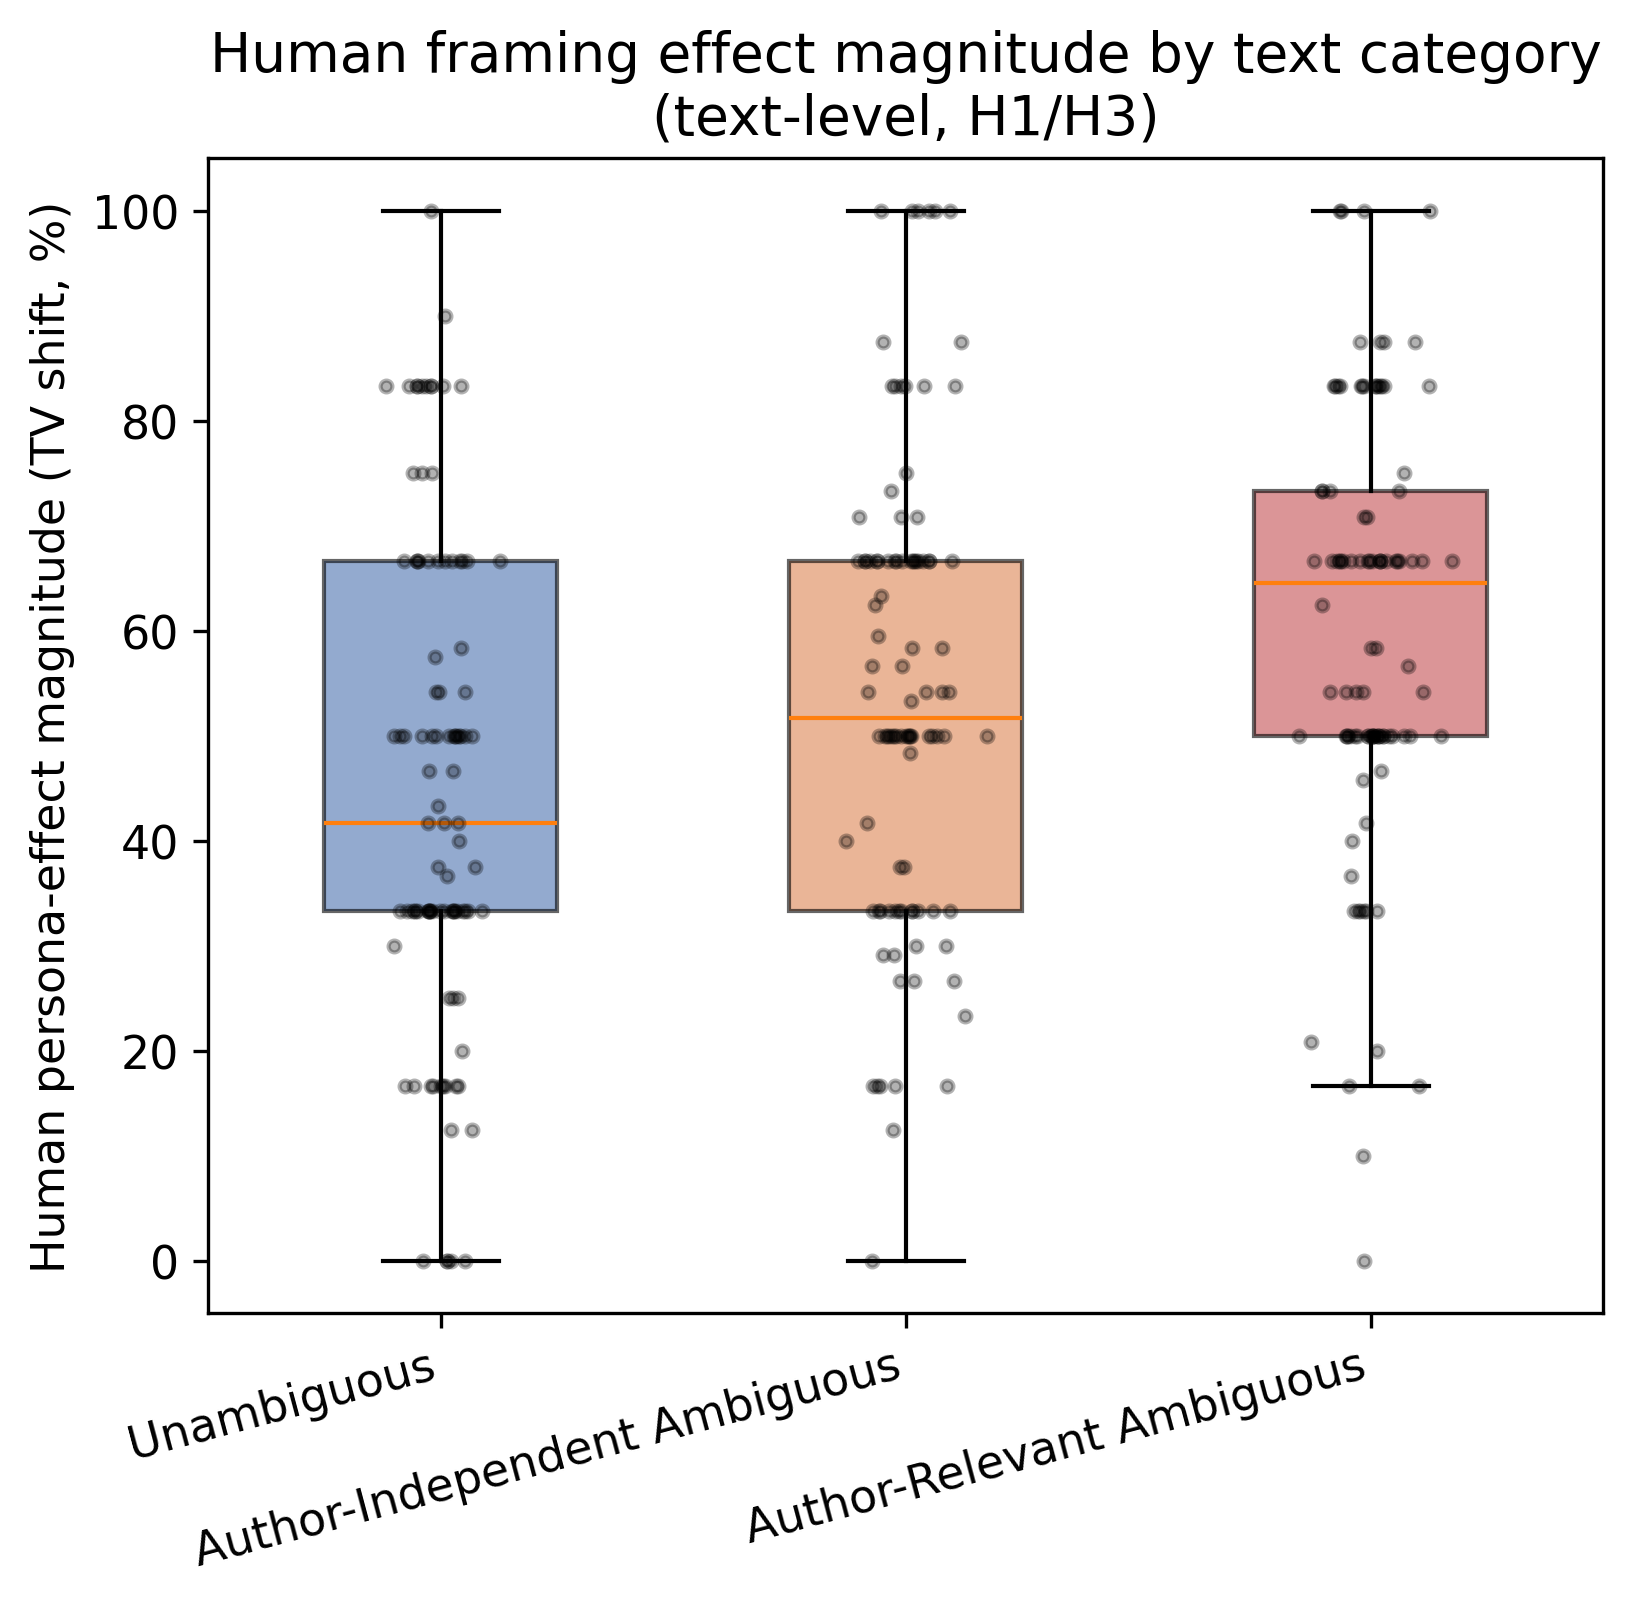
\includegraphics[width=5.0in]{images/fig01_human_tv_by_category.png}
    \caption{Human persona-effect magnitude by text category (text-level, one observation per text).}
    \label{fig:h1tv}
\end{figure}

\noindent
Mean text-level shift magnitude rises across the three categories as predicted: Unambiguous
\textbf{45.1\%} (median 41.7\%), Author-Independent \textbf{54.1\%} (51.7\%), Author-Relevant
\textbf{60.3\%} (64.6\%).

As Figure~\ref{fig:h1tv} shows, the categories overlap heavily despite this ordering. Interquartile
ranges are broad, and every category has individual texts spanning the entire range. The figure
does not show that every author-relevant text shifts more than every unambiguous one; it shows a
difference in central tendency set against considerable within-category variation.

\subsection{Permutation Test}
\label{res:h1perm}

\noindent
Given the noise floor established in Section~\ref{res:baseline_validation}, raw magnitudes
cannot be interpreted directly, so each category and persona side was tested against a
within-text permutation null (10{,}000 iterations, Holm-corrected across the six tests).

\begin{figure}[h]
    \centering
    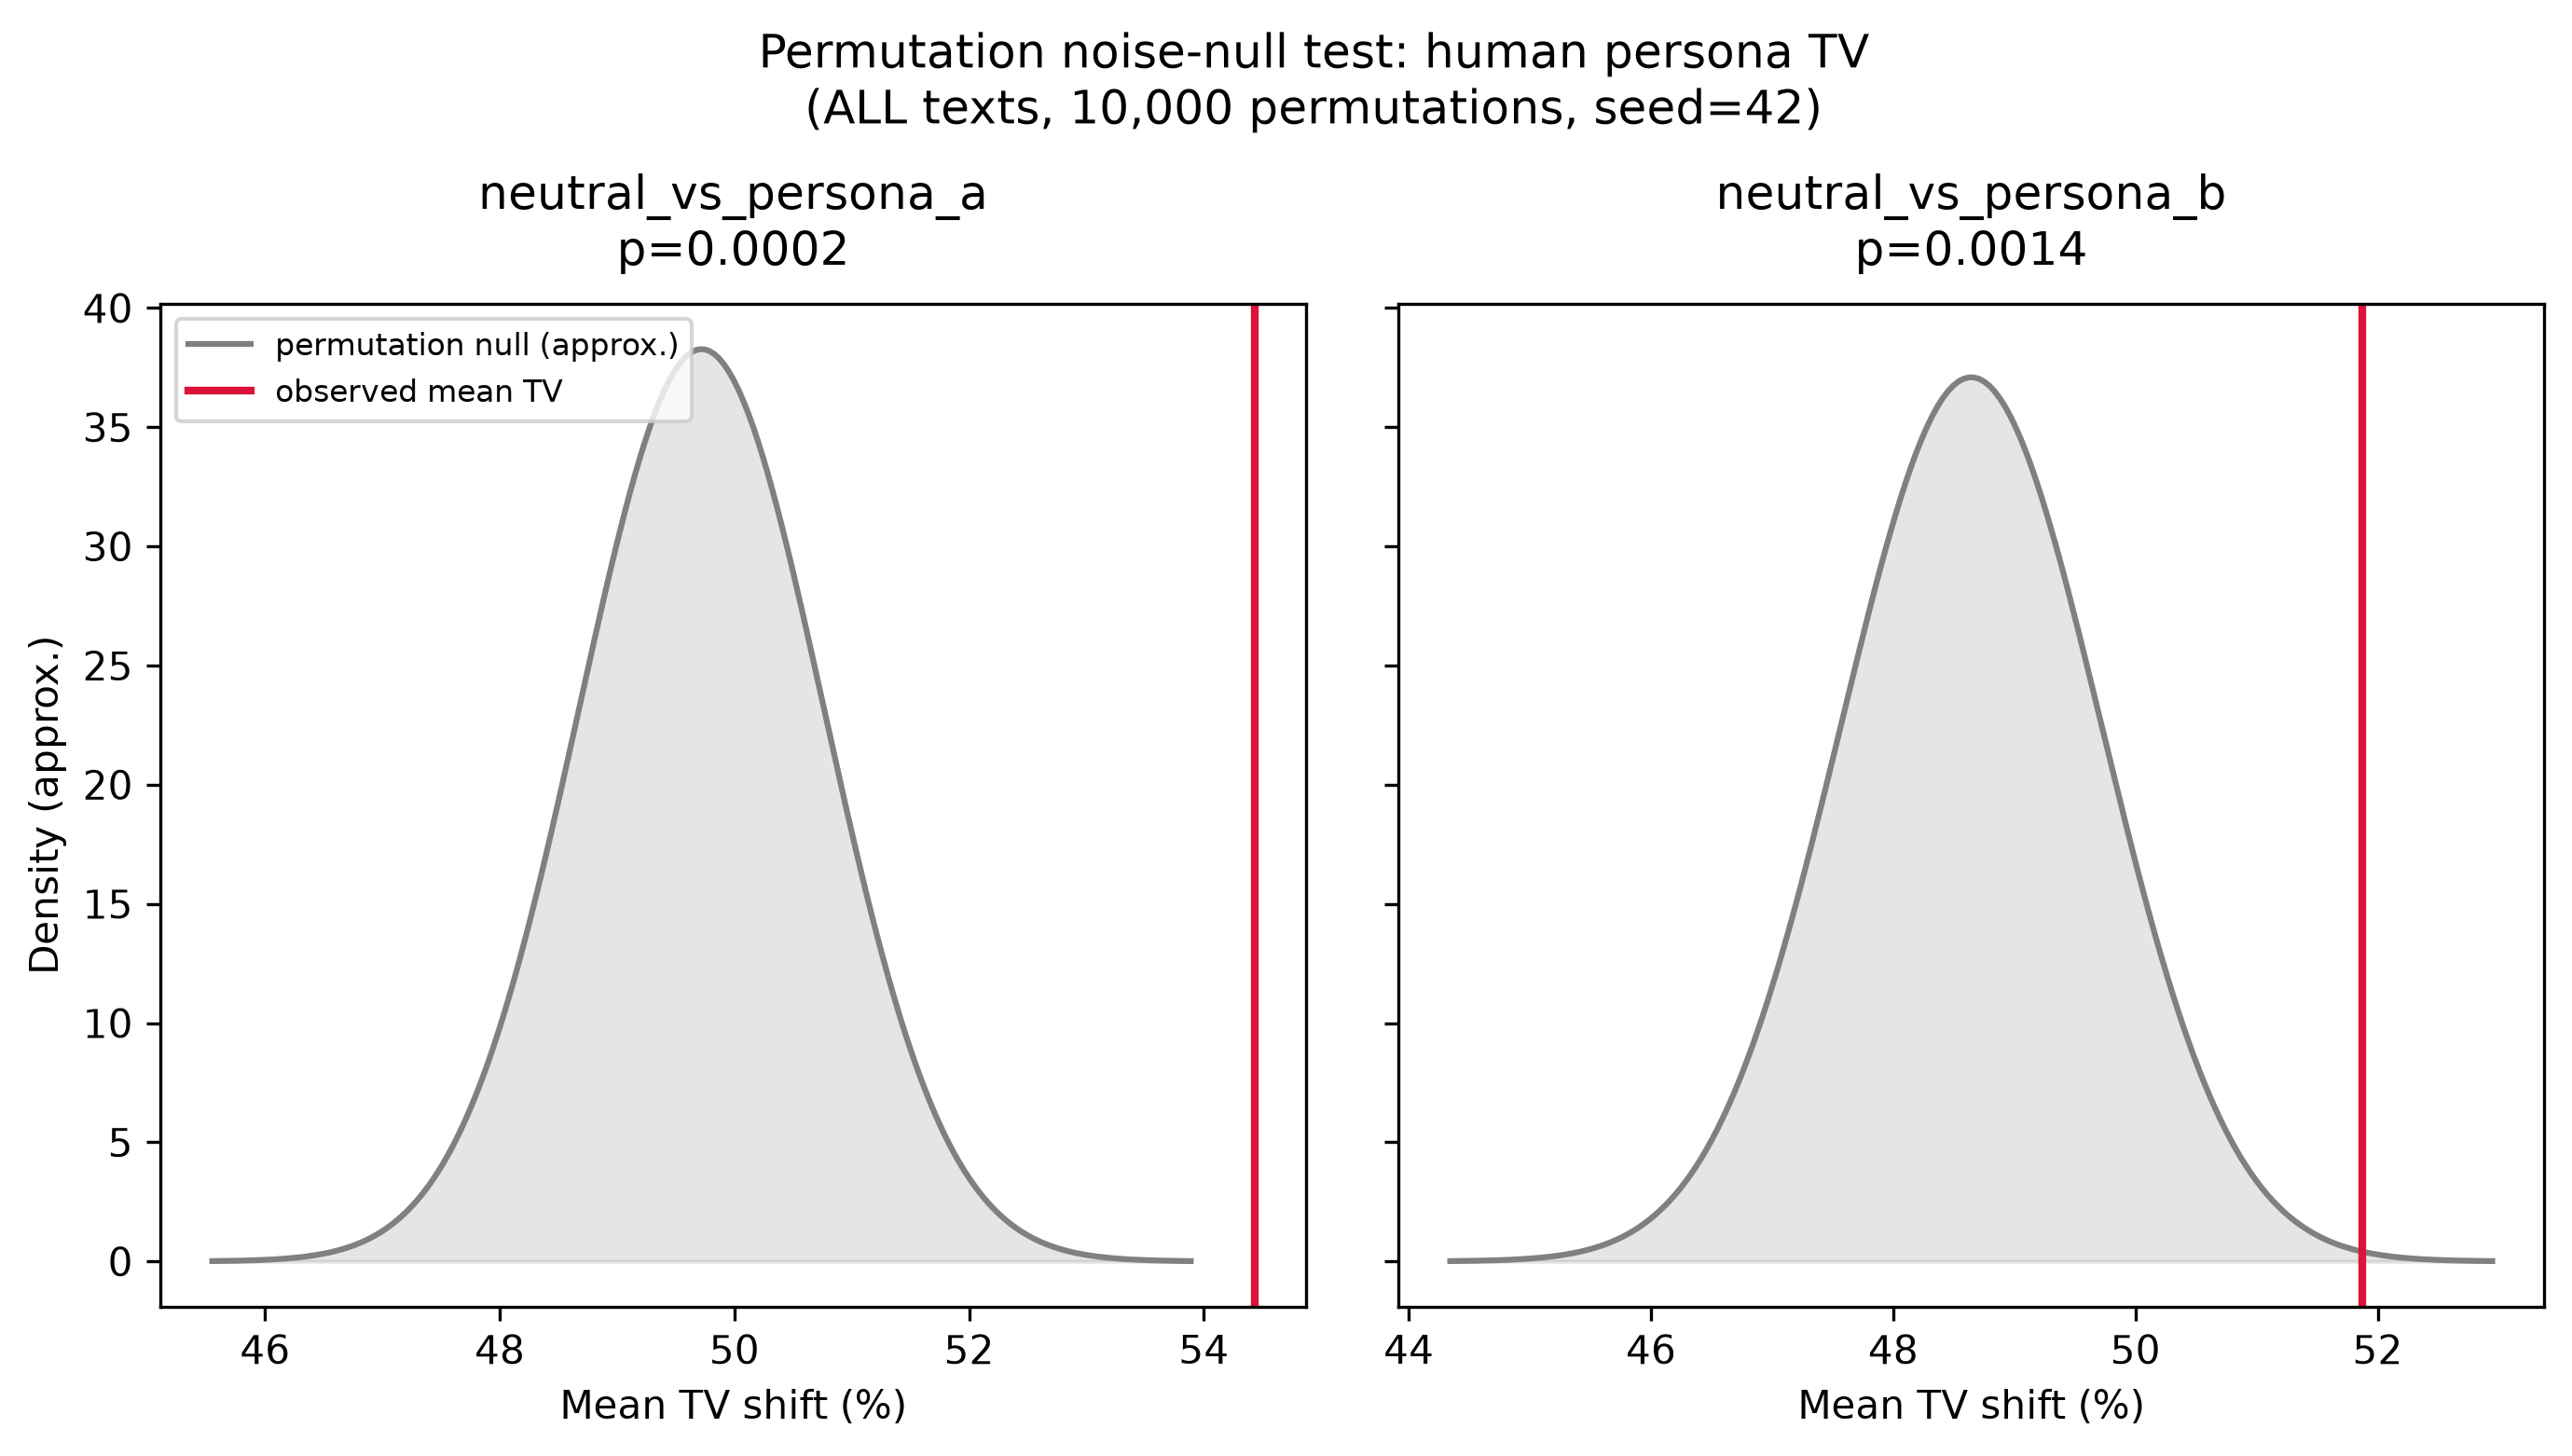
\includegraphics[width=5.0in]{images/fig03_permutation_null_human_persona.png}
    \caption{Permutation null distributions for the human persona effect, pooled across all texts, with the observed mean marked.}
    \label{fig:h1perm}
\end{figure}

\begin{table}[h]
\centering
\footnotesize
\caption{H1 permutation test results. Holm-corrected across six tests (3 categories $\times$ 2 persona sides).}
\label{tab:h1}
\begin{tabular}{lcccc}
\hline
\textbf{Category} & \multicolumn{2}{c}{\textbf{Persona side a}} & \multicolumn{2}{c}{\textbf{Persona side b}} \\
 & Observed TV & $p_{\text{Holm}}$ & Observed TV & $p_{\text{Holm}}$ \\
\hline
Author-Relevant      & 59.9\% & \textbf{0.0066} & 60.7\% & \textbf{0.0112} \\
Author-Independent   & 56.3\% & \textbf{0.0110} & 51.9\% & 0.1980 \\
Unambiguous          & 47.1\% & 0.1980          & 43.0\% & 0.2145 \\
\hline
\end{tabular}
\end{table}

\noindent
\textbf{Interpretation.} Three results are presented here, in order of evidential weight.

On author-relevant ambiguous texts the framing effect is significant on \textbf{both} persona
sides. This is what H1 predicted, and it holds.

On unambiguous control texts there is \textbf{no statistically significant} effect on either
side. That satisfies H1's control prediction, but non-rejection does not imply that the true
effect is zero, or that the manipulation worked only through author content.

For author-independent ambiguous texts, side~a crosses the significance threshold but side~b does
not. The observed shifts are 56.3\% and 51.9\%, against conditional-null means of 50.9\% and
48.9\% respectively. \emph{Significant on one side and non-significant on the other is not a test
of a difference between sides.} An exploratory direct comparison pairs each text's two raw TV
shifts: the mean A-minus-B difference is 4.44 percentage points, with a text-bootstrap
95\% interval $[-2.08, 11.06]$ points (paired sign-flip $p=0.186$; see
\texttt{results/\allowbreak author\_\allowbreak independent\_\allowbreak persona\_\allowbreak side\_\allowbreak contrast\_\allowbreak verified.csv}). The evidence on
whether \emph{each} framing effect is detectable is therefore mixed, and does not lead to a
conclusion that one persona effect is stronger than the other. This exploratory comparison is
between raw TV, not between the two separately estimated excess-over-null values.

\noindent
A cross-check makes the case for the distributional representation empirically rather than by
argument. Repeating these same six comparisons on the \emph{selected label} instead of the vote
vector (pooling each text's votes, permuting, and asking only whether the winning emotion
differs, with the identical Holm correction) yields \textbf{0 of 6} rejections under this
thesis's tie-breaking convention (a vote-share tie goes to whichever emotion is alphabetically
first). Under this conventional one-label treatment of the human data, no framing effect is
detectable at all, in any category, on either persona side. Although the respective label-change
rates are nonzero (Section~\ref{res:vectorization}), no corresponding significance test passes
once each distribution is reduced to a single winner.

\textbf{The exact count depends on the tie-breaking rule.} Ties are common at these
sample sizes, and there is no principled reason to prefer one tie-break order over another beyond
the fact that alphabetical order was the one chosen. Repeating the same selected-label test
with ties broken in reverse-alphabetical order flips the author-relevant, persona-A cell
from non-significant to significant (change rate 73.0\%, $p_{\text{Holm}} = 0.0012$), making the
overall count \textbf{1 of 6} rather than 0 of 6
(\texttt{results/\allowbreak tie\_\allowbreak break\_\allowbreak h1\_\allowbreak significance\_\allowbreak verified.csv}). This general methodological point,
that the selected-label method can at best find only a fraction of what the distributional
treatment finds, holds under either convention; the specific claim that it finds \emph{none} of
the six does not.

\noindent
\textbf{Verdict: H1 is partially supported}: supported on author-relevant texts, with no detected
effect in the unambiguous controls, and mixed for author-independent texts. This support appears
only under
the distributional treatment and is absent under the selected-label one; this is one of the
chapter's findings in its own right, taken up again in Section~\ref{res:vectorization}.

\section{H2: Author Framing Shifts Model Classifications}
\label{res:h2}

\noindent
\textbf{Hypothesis.} LLM emotion classifications will shift across author-framing conditions,
reflecting sensitivity to minimal author cues.

\subsection{Magnitude by Category and Configuration}
\label{res:h2magnitude}

\begin{figure}[h]
    \centering
    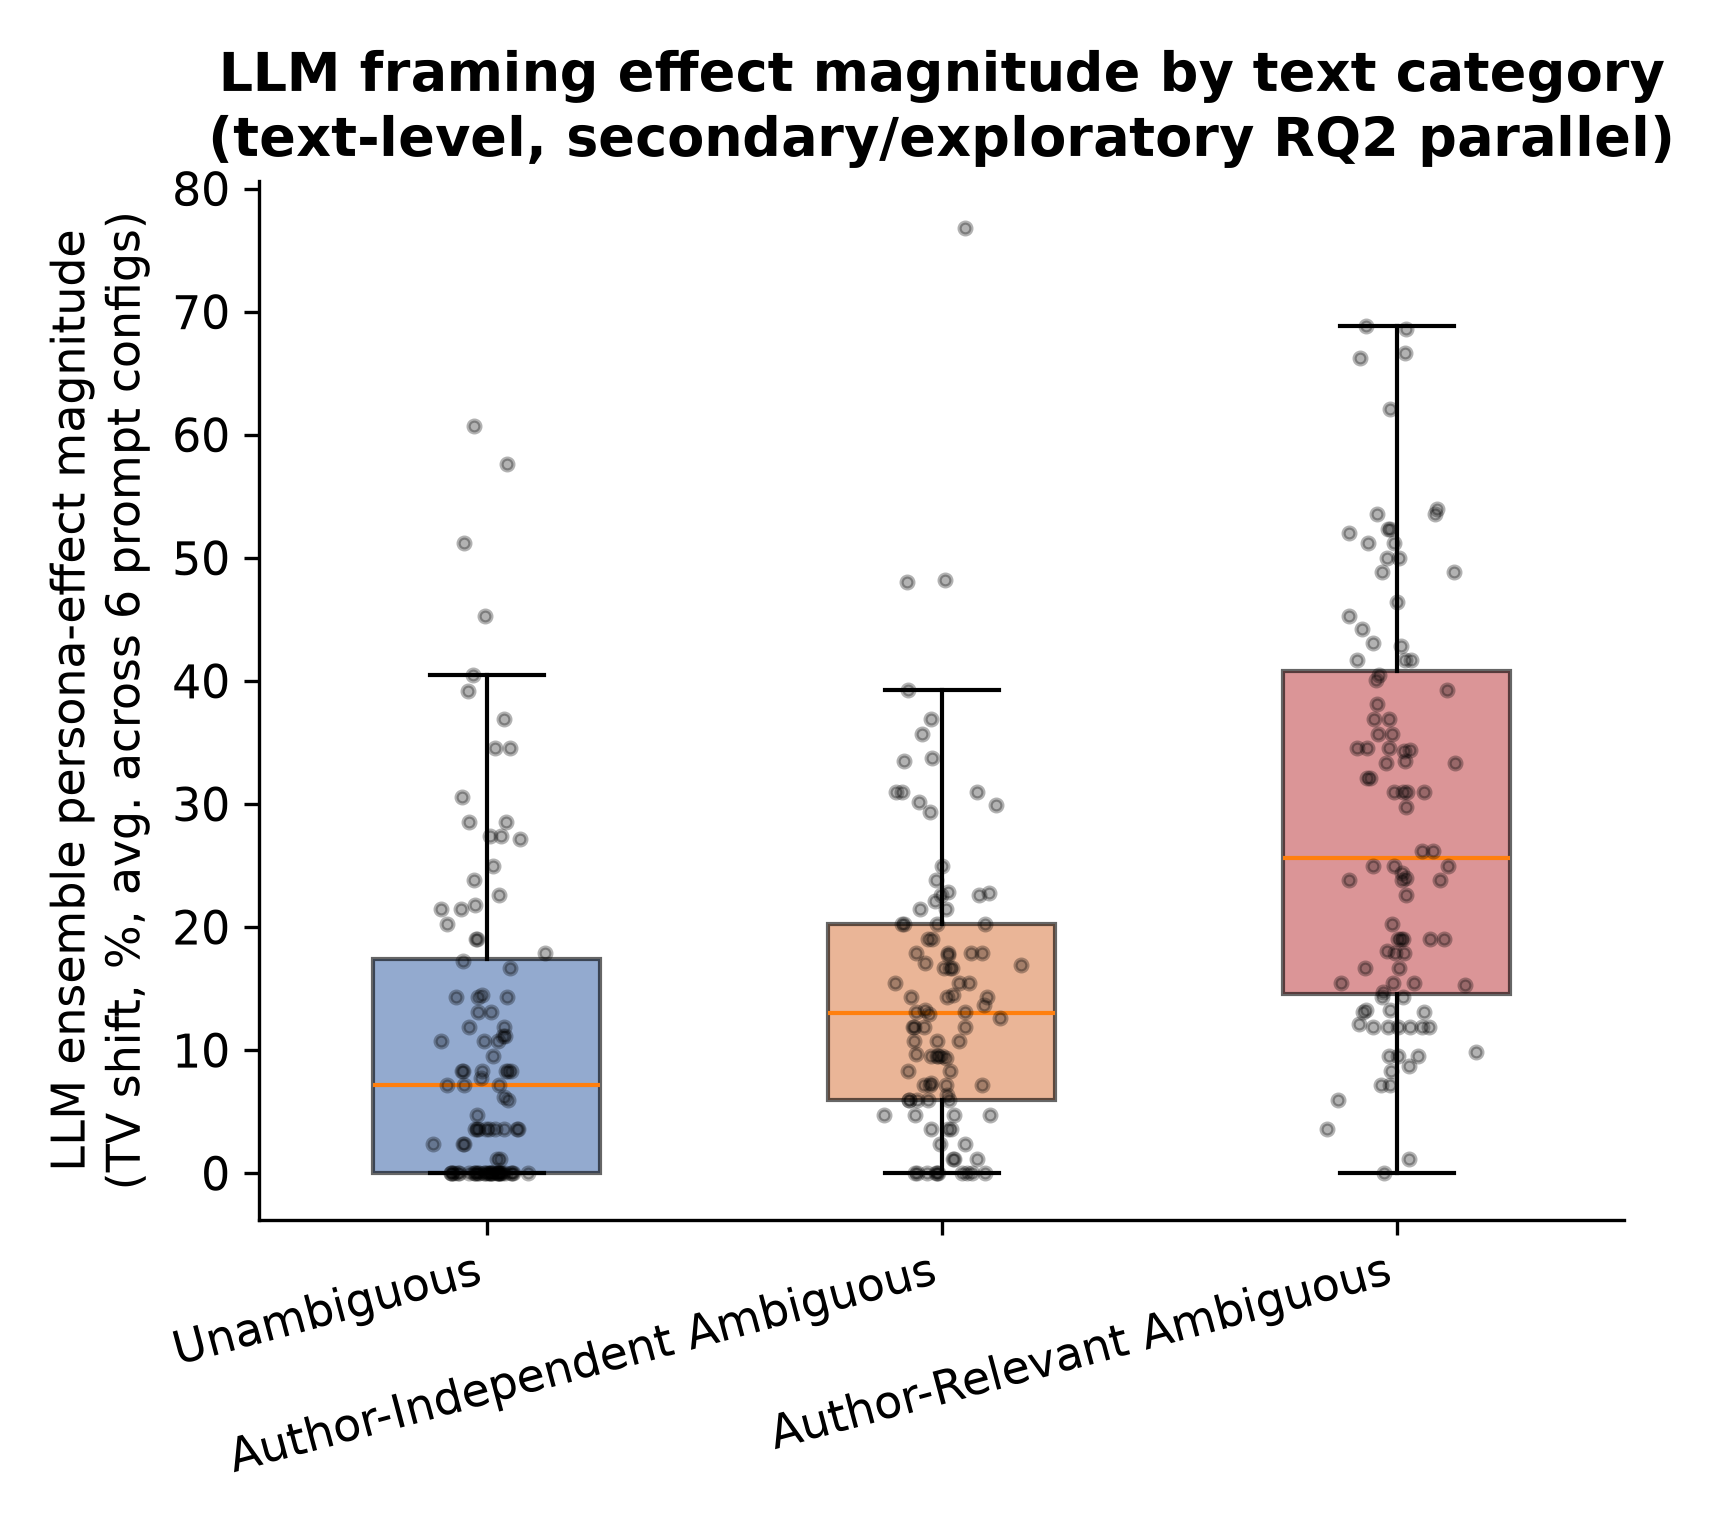
\includegraphics[width=5.0in]{images/fig02_llm_tv_by_category.png}
    \caption{Model ensemble persona-effect magnitude by text category (text-level, averaged across the six prompt configurations).}
    \label{fig:h2tv}
\end{figure}

\noindent
The mean ensemble shifts are \textbf{11.3\%} for unambiguous, \textbf{14.8\%} for
author-independent and \textbf{28.8\%} for author-relevant texts. The ordering holds for all six
prompt configurations (Figure~\ref{fig:h2config}); all seven models show a positive observed
label-change rate. The model ensemble itself is tested with the paired test below, not each
model individually.

\begin{figure}[h]
    \centering
    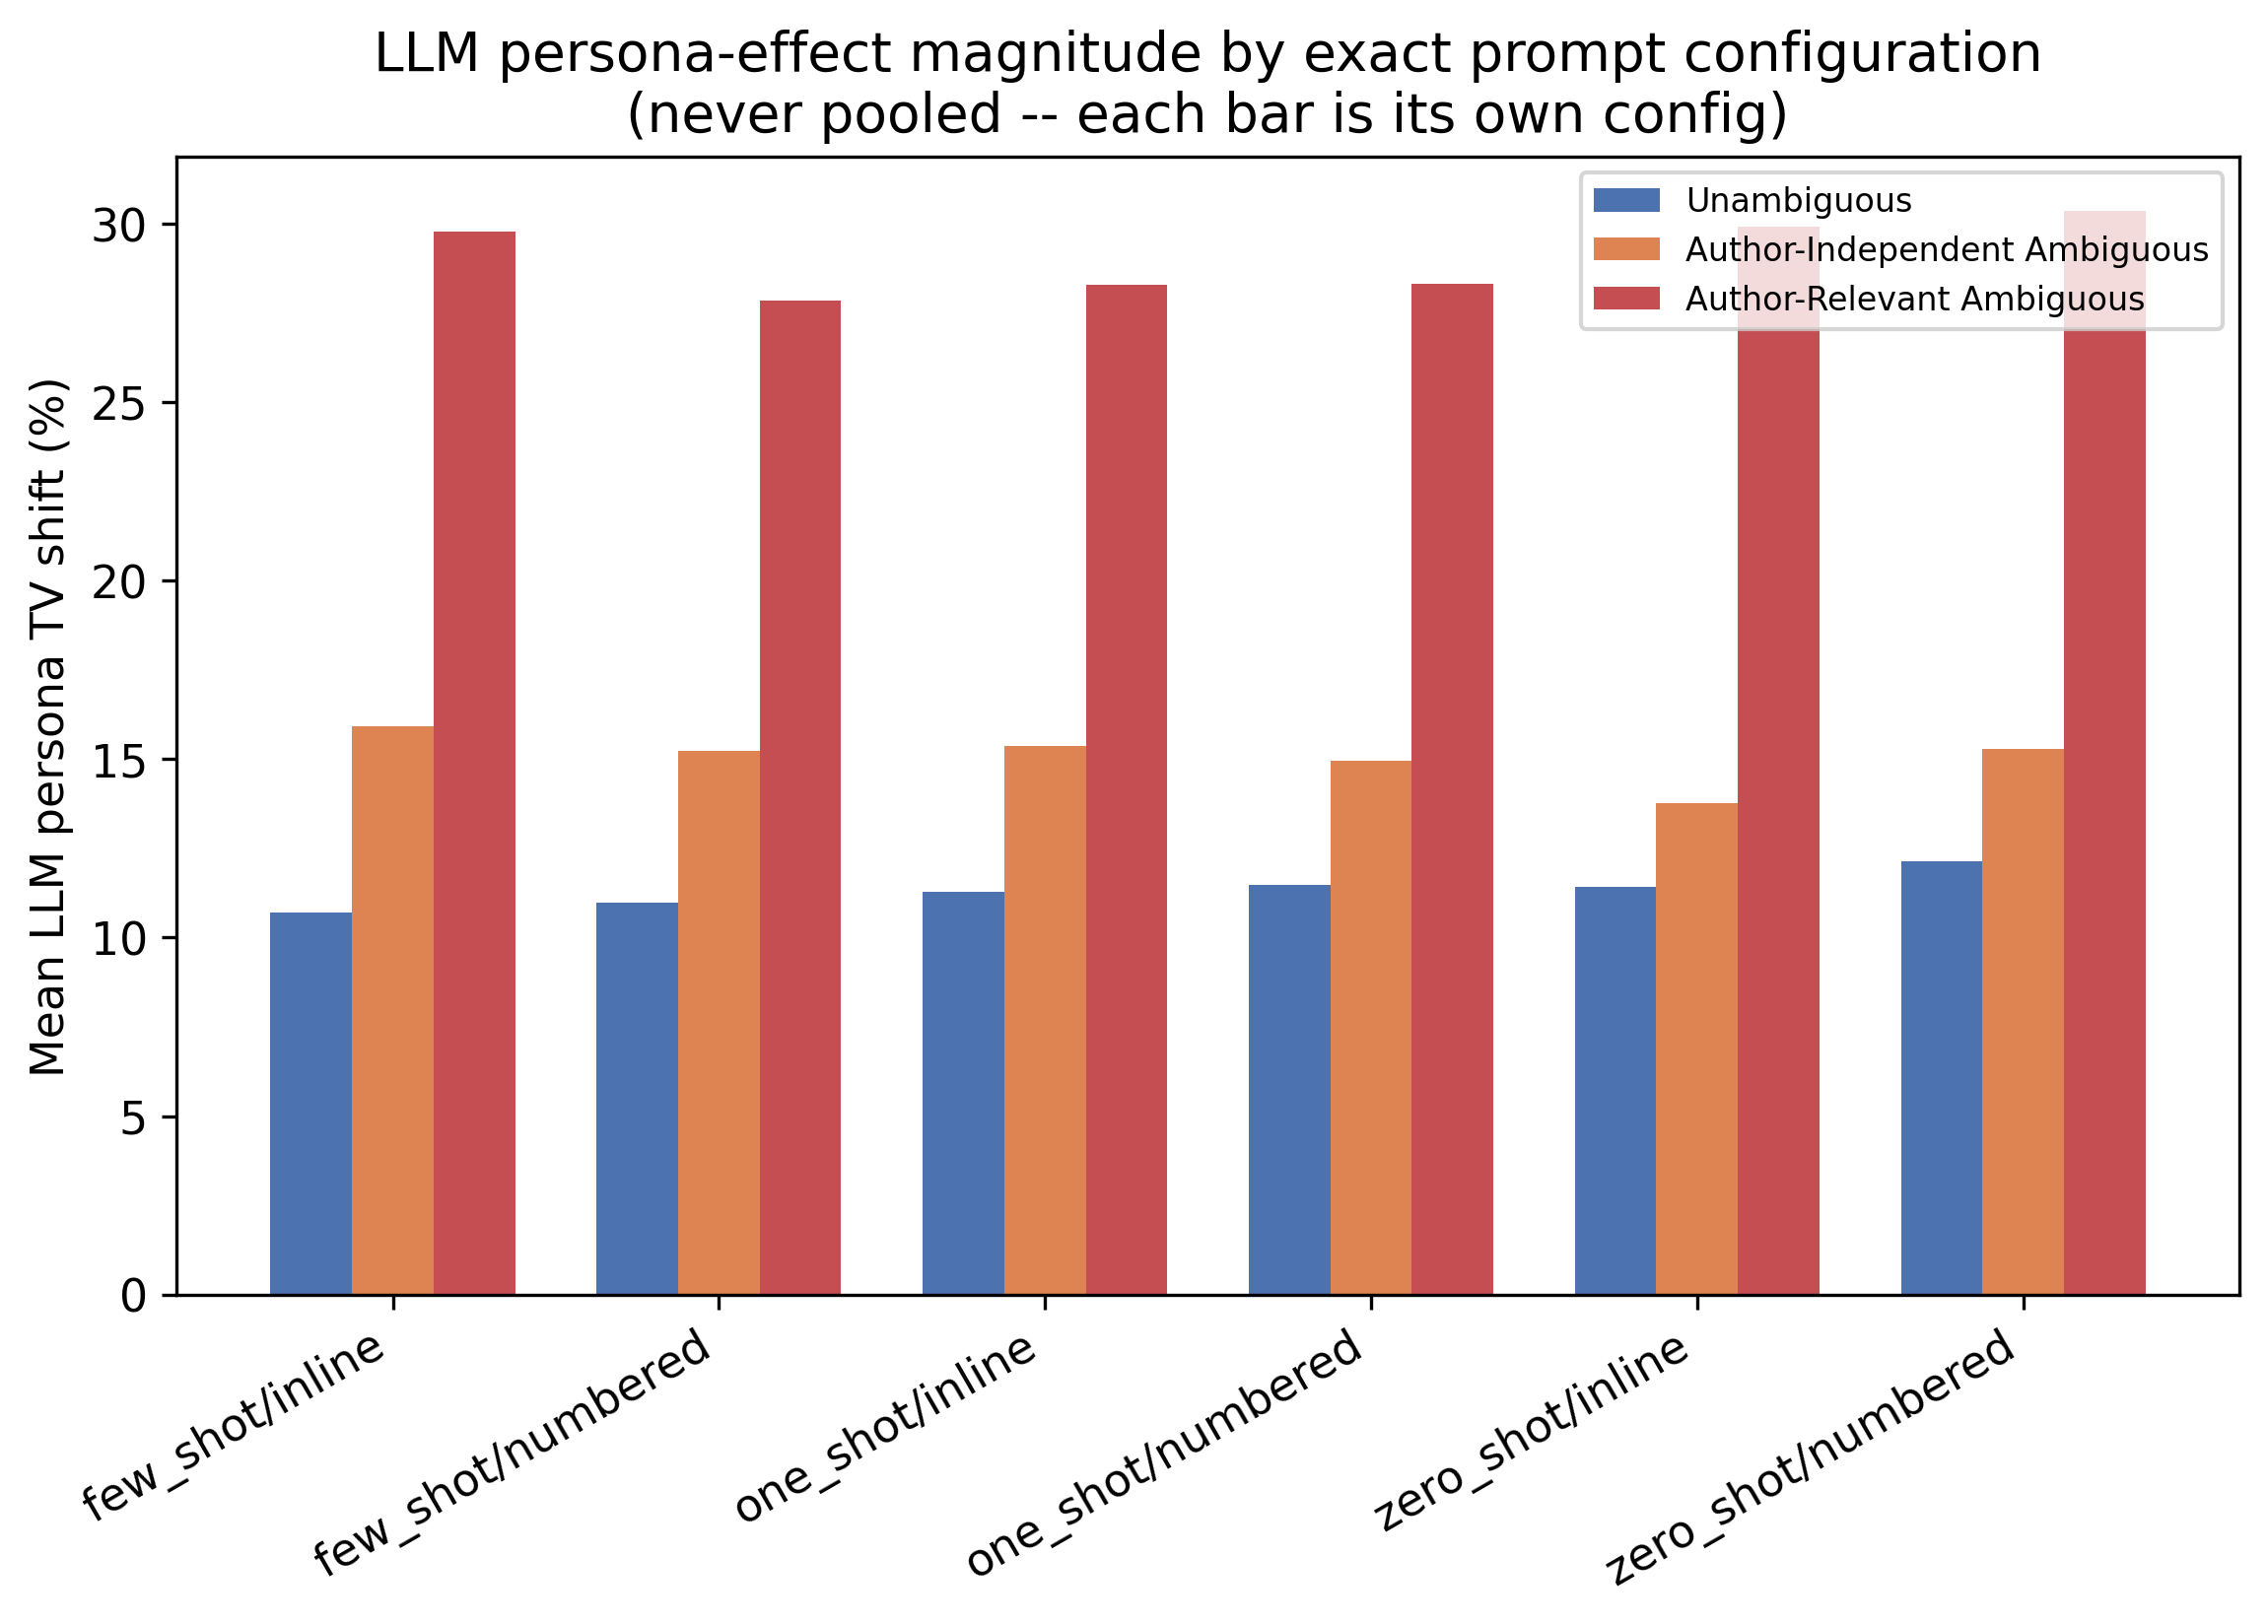
\includegraphics[width=5.0in]{images/fig04_llm_persona_by_prompt_config.png}
    \caption{Model persona effect by exact prompt configuration. Each bar is a separately computed, never-pooled comparison.}
    \label{fig:h2config}
\end{figure}

\noindent
Individual model label-change rates for author-relevant texts range from Ministral at 39.3\%
down to Gemma3 at 26.2\%. No pairwise significance test was run between models, so these are
described as highest and lowest \emph{observed} means, not as best and worst.

The shape of Figure~\ref{fig:h2tv} is strongly skewed to the right. The median ensemble shift is
substantially lower than the mean, because a large fraction of model comparisons do not shift at all
(Section~\ref{res:zeroshift}).

\subsection{Paired Permutation Test}
\label{res:h2perm}

\noindent
Because the same seven models answer both conditions, the null must hold model identity fixed
(Section~\ref{impl:permutation}). The paired sign-flip test gives:

\begin{table}[h]
\centering
\footnotesize
\caption{H2 paired sign-flip permutation test, Holm-corrected across two persona sides.}
\label{tab:h2}
\begin{tabular}{lccc}
\hline
\textbf{Comparison} & \textbf{Observed mean TV} & \textbf{95\% CI (text-clustered)} & $p_{\text{Holm}}$ \\
\hline
Neutral vs persona a & 16.80\% & [14.74, 18.97] & \textbf{0.0002} \\
Neutral vs persona b & 19.78\% & [17.50, 22.08] & \textbf{0.0002} \\
\hline
\end{tabular}
\end{table}

\subsection{What This Test Does and Does Not Establish}
\label{res:h2scope}

\noindent
The statistic is TV between ensemble vectors, so the test detects \textbf{coordinated net
redistribution} across models. It does not measure whether any individual model changed its
answer, and that difference has real consequences.

Under a paired sign flip, concordant model pairs cancel and only discordant pairs contribute. When
a cell contains exactly one discordant model, its TV equals $1/n$ under \emph{every} possible
swap: the null is a point mass, and the test cannot reject, regardless of how real the change is. In these data, 37.9\% of cells have no discordant model and a further 23.3\%
have exactly one, so \textbf{61.2\% of cells contribute no variance to the null}. The remaining
38.8\% drive the test.

Because of this, the complementary quantity is reported as well: of 24{,}736 valid model pairs,
\textbf{5{,}263 (21.3\%) changed their label} between conditions. H2 as worded is supported by
both measures, but they answer different questions and only the first is what the $p$-value refers
to.

\noindent
Unlike H1, H2's verdict does not depend on the choice of representation: the same selected-label
cross-check described in Section~\ref{res:h1perm} also rejects the null on both persona sides
under the old, one-label treatment ($p_{\text{Holm}} = 0.0002$ for both). The model-side selected-label
test survives aggregation to a single winner, whereas most of the human selected-label tests do
not. This is not because of a smaller human raw change rate: at the label level, humans change
their selected answer far more often than the model ensemble does (52.8\% of human comparisons
versus 18.4\% of model comparisons, Table~\ref{tab:vectorization}). The
human tests are underpowered relative to the model tests, most plausibly because each human cell
casts only three votes against the model ensemble's much larger effective sample, not because the
human effect is genuinely smaller.

\noindent
\textbf{Verdict: H2 is supported} on both persona sides.

\section{Is It the Persona, or Merely Having an Author?}
\label{res:generic}

\noindent
Each comparison of a neutral to a persona condition carries a confound: persona prompts add an
author line that neutral prompts lack entirely. A measured shift could reflect the persona's
content or merely the presence of an attribution. The \texttt{generic\_human} condition separates
them.

\begin{table}[h]
\centering
\footnotesize
\caption{Decomposition of the model framing effect using the generic-human control. Each row uses
only the models that answered validly under all three of the neutral, generic-human and persona
conditions for that side (a three-way intersection, stricter than matching models pairwise), so
the two component distances and the confounded distance are computed over the same model set.}
\label{tab:generic}
\begin{tabular}{lccc}
\hline
\textbf{Comparison} & \textbf{Side a} & \textbf{Side b} & \textbf{95\% CI (a / b)} \\
\hline
Neutral $\rightarrow$ generic human & \textbf{7.98\%} & \textbf{8.01\%} & [7.23, 8.75] / [7.26, 8.77] \\
Generic human $\rightarrow$ specific persona & \textbf{16.20\%} & \textbf{19.30\%} & [14.14, 18.33] / [17.01, 21.61] \\
Neutral $\rightarrow$ persona \emph{(confounded)} & 16.73\% & 19.78\% & [14.68, 18.89] / [17.50, 22.08] \\
\hline
\end{tabular}
\end{table}

\noindent
\textbf{Interpretation.} A generic author line on its own produces a shift of almost exactly the
same size on both sides (7.98\%--8.01\%). That is not negligible: naming any author at all
changes how the models classify. The effect of the persona's specific content, measured with the
author line held constant, is roughly twice as large on both sides, and about as large as the
full confounded comparison. These three distances describe what is associated with each step
under matched models; they are not claimed to be additive components of one total effect.

The persona-content step is the larger of the two measured distances on both sides, while the
author-line-alone step is smaller but still non-negligible. The approved proposal did not specify
this decomposition, so the analysis is labelled secondary. Still, it turns a limitation that could
otherwise only be acknowledged into one that is measured.

\section{H3: Framing Effects and Ambiguity Type}
\label{res:h3}

\noindent
\textbf{Hypothesis.} Framing effects will be stronger for author-relevant ambiguous texts than for
author-independent ambiguous texts.

\subsection{Raw Contrasts}
\label{res:h3raw}

\noindent
Each text is reduced to a single number, its mean shift over the two persona sides, and the three
categories are compared pairwise. The permutation null shuffles which category each text's number
belongs to; the effect size is the raw difference in mean shift, and its confidence interval is a
text-level bootstrap.

\begin{table}[h]
\centering
\footnotesize
\caption{H3 pairwise contrasts on raw TV, Holm-corrected across the three contrasts.}
\label{tab:h3raw}
\begin{tabular}{lccc}
\hline
\textbf{Contrast} & \textbf{Difference} & \textbf{95\% CI} & $p_{\text{Holm}}$ \\
\hline
Author-Independent vs Unambiguous     & 9.04pp  & $[2.63, 15.33]$ & 0.0144 \\
Author-Relevant vs Author-Independent & 6.18pp  & $[0.30, 12.08]$ & 0.0403 \\
Author-Relevant vs Unambiguous        & 15.22pp & $[9.08, 21.29]$ & 0.0003 \\
\hline
\end{tabular}
\end{table}

\noindent
In raw terms, all three contrasts are significant after correction. However, the contrast H3 is
actually about, author-relevant versus author-independent, is the \textbf{weakest of the three}:
it has the smallest difference, the widest relative confidence interval and the largest corrected
$p$-value. It is not a dramatic separation, and, as Section~\ref{res:h3null} shows next, this
specific contrast does not survive being referenced against each text's own sampling null, so
``significant in raw terms'' is the most this result supports on its own.

\subsection{Referencing Against Each Text's Own Sampling Null}
\label{res:h3null}

\noindent
The raw comparison is complicated by a property of small-sample TV. As set out in
Section~\ref{impl:nullref}, TV between two three-vote samples is not zero under no effect, and it
increases with the dispersion of the underlying distribution. The ambiguous categories are by
construction the dispersed ones. A raw category comparison is therefore a combination of baseline
dispersion and the framing effect.

\begin{table}[h]
\centering
\footnotesize
\caption{Observed, expected-under-null, and excess TV by category (human, text-level).}
\label{tab:h3excess}
\begin{tabular}{lccc}
\hline
\textbf{Category} & \textbf{Observed TV} & \textbf{Expected under sampling null} & \textbf{Excess} \\
\hline
Unambiguous & 45.07\% & 43.07\% & \textbf{2.00pp} \\
Author-Independent & 54.10\% & 49.90\% & \textbf{4.20pp} \\
Author-Relevant & 60.28\% & 54.59\% & \textbf{5.70pp} \\
\hline
\end{tabular}
\end{table}

\noindent
The expected null TV is \emph{itself} strongly ordered by category, ranging from roughly 43\% to
55\%. Once each text is referenced against its own null, the excess above that conditional-null
expectation is on the order of two to six percentage points rather than forty-five to sixty.

\begin{table}[h]
\centering
\footnotesize
\caption{H3 contrasts on raw TV versus null-referenced excess TV.}
\label{tab:h3compare}
\begin{tabular}{lcc}
\hline
\textbf{Contrast} & \textbf{Raw} & \textbf{Null-referenced} \\
\hline
Author-Relevant $-$ Author-Independent & 6.18pp, $p_{\text{Holm}} = 0.040$ & 1.49pp, $p_{\text{Holm}} = 0.697$ \\
Author-Independent $-$ Unambiguous & 9.04pp, $p_{\text{Holm}} = 0.014$ & 2.21pp, $p_{\text{Holm}} = 0.697$ \\
Author-Relevant $-$ Unambiguous & 15.22pp, $p_{\text{Holm}} = 0.0003$ & 3.70pp, $p_{\text{Holm}} = 0.287$ \\
\hline
\textbf{Holm-significant} & \textbf{3 of 3} & \textbf{0 of 3} \\
\hline
\end{tabular}
\end{table}

\noindent
\textbf{Interpretation, stated carefully.} The ordering is preserved in direction under
null-referencing (2.00 $<$ 4.20 $<$ 5.70), but none of the three contrasts remains
significant after correction.

Three separate conclusions follow, and they should be kept apart.

First, the raw contrasts show an observed difference of the kind the approved proposal
anticipated. H3's predicted ordering \emph{is} present in observed shift magnitude.

Second, non-significance under null-referencing does not mean that the categories are equivalent.
The excess-TV estimator subtracts an estimated conditional-null quantity, and the resulting point
estimates are considerably smaller (1.49--3.70pp) than the raw estimates (6.18--15.22pp), while
the confidence intervals are, if anything, slightly tighter in absolute width than the raw contrasts'
intervals (about 8.6--9.5pp wide versus 11.8--12.7pp raw). None of the three reaches significance
because the estimated excess itself is small relative to that width, not because the interval has
widened. Absence of evidence is not evidence of absence.

Third, excess TV measures observed distance above the chosen conditional-null expectation; it is a
useful sensitivity statistic, not a validated decomposition into causal framing and baseline-noise
components, since the pooled votes it refers to include observations from both conditions, and the
spread of those votes could itself reflect condition differences. What it does show is that, given
this reference, the category contrast becomes small and statistically inconclusive, so the raw
ordering is sensitive to the choice of analytical reference, and this study cannot cleanly
separate framing from baseline dispersion at 100 texts per category. These data therefore do not
support a strong behavioural reading of the raw ordering.

This analysis was specified only after the raw result was known. It is therefore reported as a
sensitivity analysis next to the raw contrasts, not in place of them; making it primary would
amount to choosing an analysis by its outcome.

\noindent
\textbf{Verdict: H3 shows the predicted raw ordering, but the framing-specific contrast is
inconclusive after referencing baseline vote dispersion.} The point should be stated as an
ordering in observed disagreement, not as a demonstrated framing-sensitivity gradient. Recall
also from Section~\ref{meth:ambiguity} that the categories were partly defined using an LLM
judge's own sensitivity to author-relevance, which makes H3 a transfer comparison rather than an
independent discovery of that grouping principle.

\section{H4: Human--Model Alignment}
\label{res:h4}

\noindent
\textbf{Hypothesis.} The direction of framing-induced shifts in LLM classifications will partially
align with human judgment shifts, but the magnitude of these shifts will differ.

Each component predicts something different, and either can hold without the other, so testing
proceeds separately for each.

\subsection{Magnitude}
\label{res:h4magnitude}

\noindent
Two questions are easily confused here, and they must be kept apart.

\textbf{Is there a covariation} between shifts in humans and shifts in models? The 300 text-level
means are used to compute Spearman's $\rho = 0.331$, 95\% CI $[0.223, 0.428]$; both persona sides
are averaged on the human side, and both sides and six configurations are averaged on the model
side (text bootstrap; Figure~\ref{fig:h4scatter}). The calculation is recorded in
\texttt{results/\allowbreak h4\_\allowbreak text\_\allowbreak level\_\allowbreak covariation\_\allowbreak verified.csv}. This positive relationship indicates
nothing about the equality of the two magnitudes.

\begin{figure}[h]
    \centering
    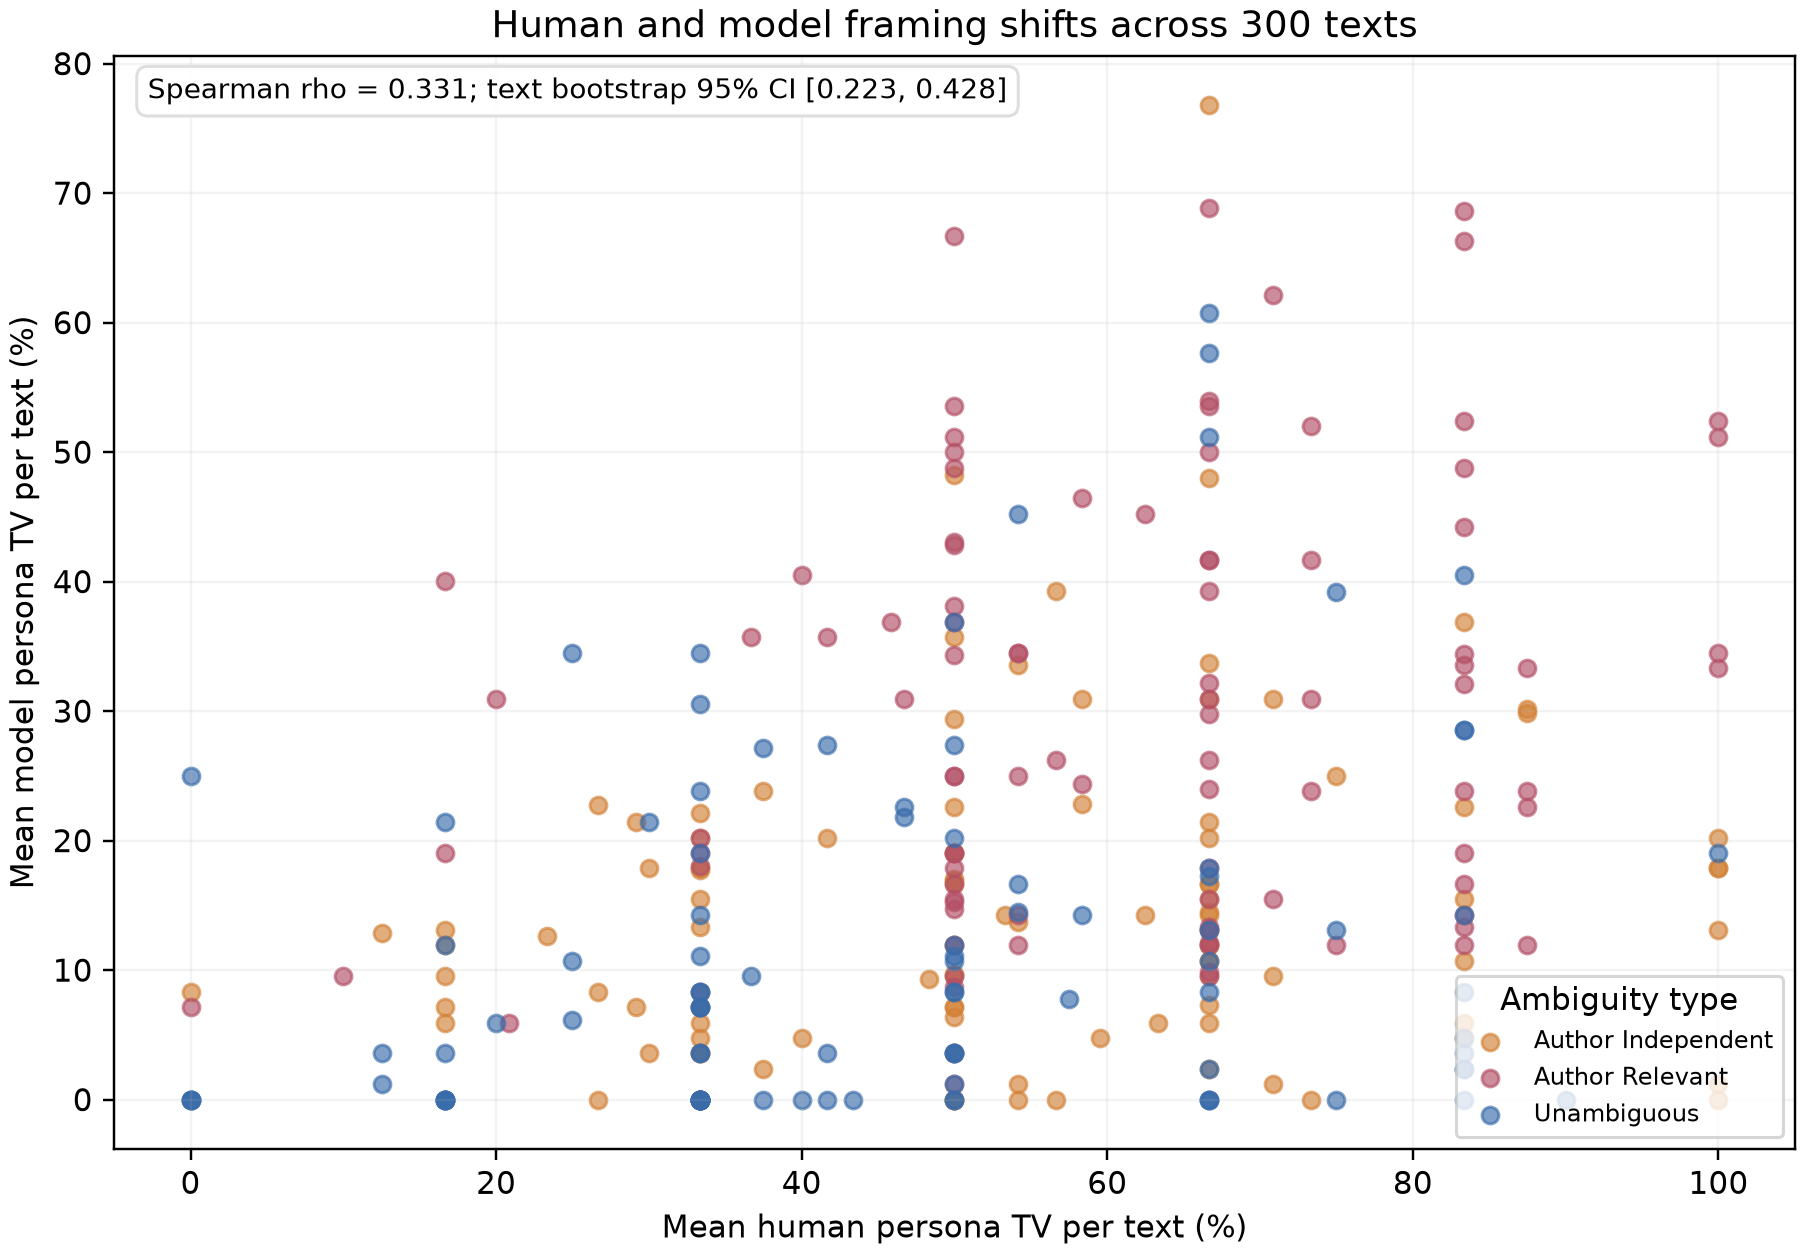
\includegraphics[width=5.0in]{images/fig05_human_llm_magnitude_scatter.png}
    \caption{Mean human versus mean model shift magnitude for each of 300 texts, coloured by category.}
    \label{fig:h4scatter}
\end{figure}

\textbf{Difference} asks whether the sizes differ, and this is what H4 actually predicts. A
paired Wilcoxon signed-rank test over 300 text-level pairs gives a mean paired difference of
\textbf{34.86pp} (human minus model), 95\% CI $[32.23, 37.54]$, $p = 4.68\times10^{-48}$, with
matched-pairs rank-biserial $r = 0.978$, close to the theoretical maximum, so that human shift is
greater than model shift for almost all texts, not just on average (279 of 300 texts shift in
that direction, 16 the other, 5 tied).

\subsection{Is the Magnitude Gap an Artefact of Vote Counts?}
\label{res:h4counts}

\noindent
Human vectors are built from three raters and model vectors from as many as seven models. Some
of the difference might be arithmetic rather than behavioural: TV depends partly on the number of
votes behind each vector. Rather than argue the point, this was tested directly.

The number of votes was fixed at three on both sides: human votes were subsampled to three per
condition, and the \emph{same three model identities} were drawn for the neutral and persona
sides of each cell, holding ensemble composition fixed as well as size. Two hundred independent
draws per comparison were performed, with the point estimate an equal-weight average across the
balanced category $\times$ side $\times$ configuration strata.

\begin{table}[h]
\centering
\footnotesize
\caption{Magnitude gap before and after standardising both sides to three votes.}
\label{tab:h4counts}
\begin{tabular}{lc}
\hline
 & \textbf{Mean human $-$ model gap} \\
\hline
Unmatched & 34.86pp \\
Count-standardised (3 votes vs the same 3 models) & \textbf{$\approx$33pp} \\
\hline
Reduction from count standardisation & $\approx$1.5pp (about 4\% of the raw gap) \\
\hline
\end{tabular}
\end{table}

\noindent
\textbf{A note on precision.} The standardised figure is a Monte Carlo estimate made with 200
draws per comparison, and is quoted deliberately as \emph{approximately} 33 percentage points
rather than to two decimals.

When the same inputs and the same seed are used, the same estimate is obtained to six decimal
places on repeated runs. The \emph{ordering} of votes within a cell is what makes it move
slightly. Subsampling draws indices, so if a condition has more than three votes, the same
multiset presented in a different order yields a different sampled subset under the same seed.
Re-ordering the votes within each cell, sorting or reversing them while leaving the multiset
untouched, moves the estimate between 33.34 and 33.37pp, and five independent seeds span 33.32 to
33.37pp.

That range, roughly 0.04pp either side, is about where a one-decimal figure rounds up or down, so
no decimal is claimed. This is not crucial to the interpretation: count standardisation reduces
the estimated gap by about 1.5 percentage points for all orderings and all seeds tested.

\noindent
\textbf{Interpretation.} Standardising both sides to the same number of votes cast reduces the
estimated gap from 34.86 to approximately 33 percentage points, a decrease of about 1.5 points
(4\%), and the gap remains within each of the categories. In line with the precision noted above,
this is expressed to the nearest whole point, not to two decimal places, since the second decimal
place moves by more than that between orderings and seeds. This procedure is limited in that it
does not causally identify the proportion of the gap explained by vote counts, and it does not
remove the between-person/within-model design asymmetry discussed below: humans still shift
substantially more than the model ensemble, and this is not an artefact of counting.

Count standardisation leaves two qualifications untouched. The human comparison is
\textbf{between-person} (different raters in each condition) and the model comparison is
\textbf{within-model}, with the same model answering both conditions. Part of the human change is
thus between-rater variability for which there is no model counterpart. And each model produced
only one generation per condition, so model-side stochastic variability is unmeasured.

\subsection{Direction}
\label{res:h4direction}

\begin{figure}[h]
    \centering
    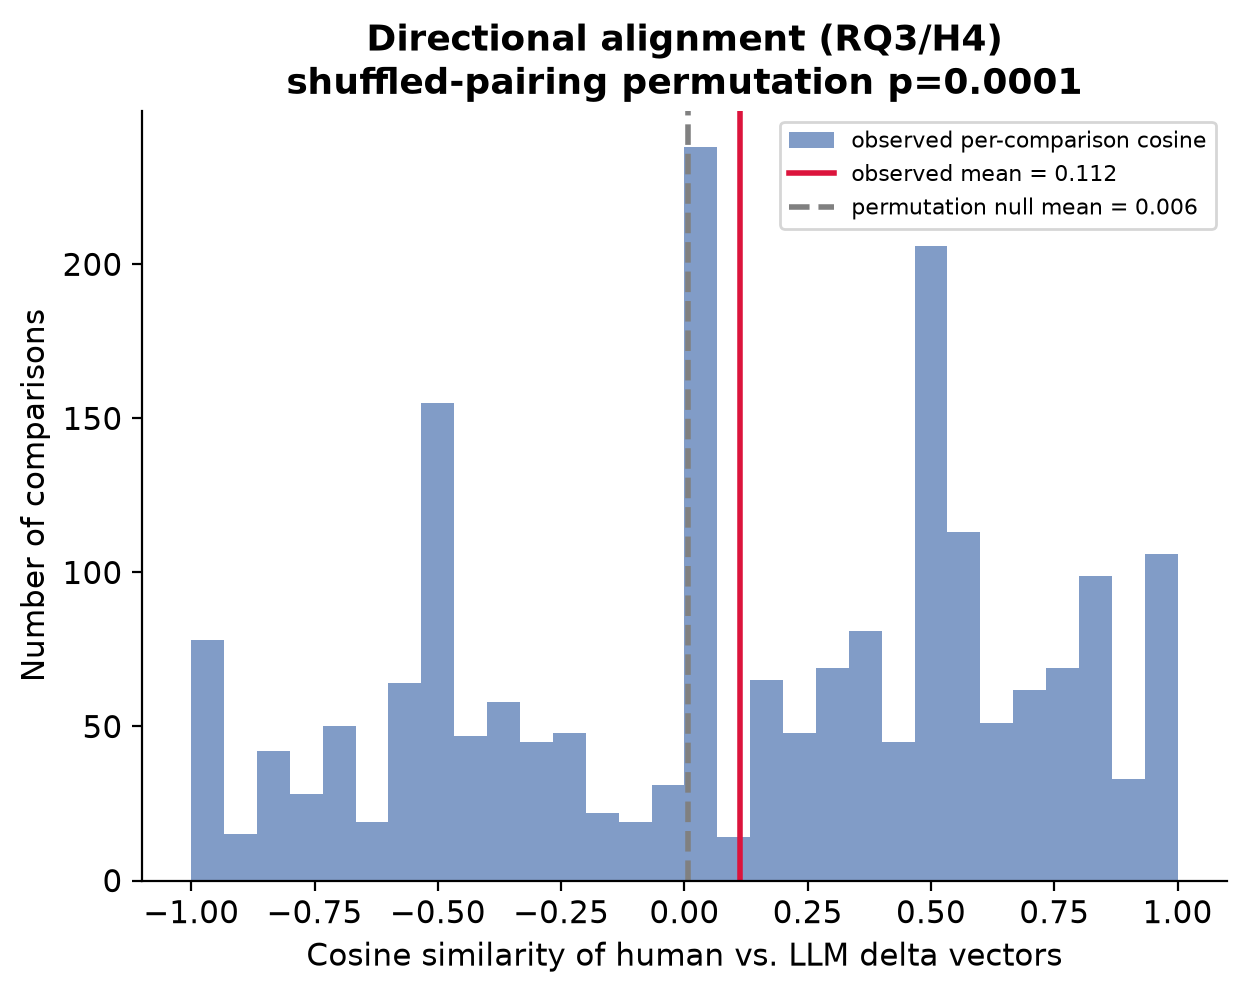
\includegraphics[width=5.0in]{images/fig06_directional_cosine_alignment.png}
    \caption{Distribution of per-comparison directional cosine between human and model delta vectors, one point per (text, side, prompt-configuration) comparison, with the observed mean and the chance-pairing null marked.}
    \label{fig:h4cosine}
\end{figure}

\noindent
Mean cosine between human and model delta vectors is \textbf{0.112}, 95\% CI $[0.072, 0.152]$,
against a shuffled-pairing permutation null (mean $0.006$), $p = 0.0001$. The direction of the
model ensemble shift is thus more closely associated with the direction of the corresponding
human shift for the text than random pairing would produce, but a cosine of about 0.11 is a
weak, partial association, not a close match.

\textbf{Coverage.} This is calculated at the individual comparison (per text, per side, per
prompt-configuration) level throughout, not as an average over a coarser, per-text level. Of the
3{,}600 total such comparisons, \textbf{2{,}020 (56\%)} are defined, and 252 of the 300 texts
(84\%) have at least one defined comparison among their set of twelve. Comparisons with no
direction to compare are called undefined and are not treated as zero.

\noindent
\textbf{Verdict: H4 is partially supported.} The magnitude component is \textbf{supported}: the
magnitudes differ, substantially and robustly to count standardisation, as H4 predicts. The
direction component is \textbf{partially supported}: alignment is above chance but weak, which is
the literal meaning of H4's word ``partially''.

The direction analysis is not immune to small-sample noise either. Cosine is invariant to
multiplying a vector by a positive scalar, but drawing three votes rather than seven is not
scalar multiplication: it can change a delta's direction, and it can make the delta exactly zero,
in which case direction becomes undefined rather than being preserved.

\section{Where the Probability Mass Moved}
\label{res:emotions}

\begin{figure}[h]
    \centering
    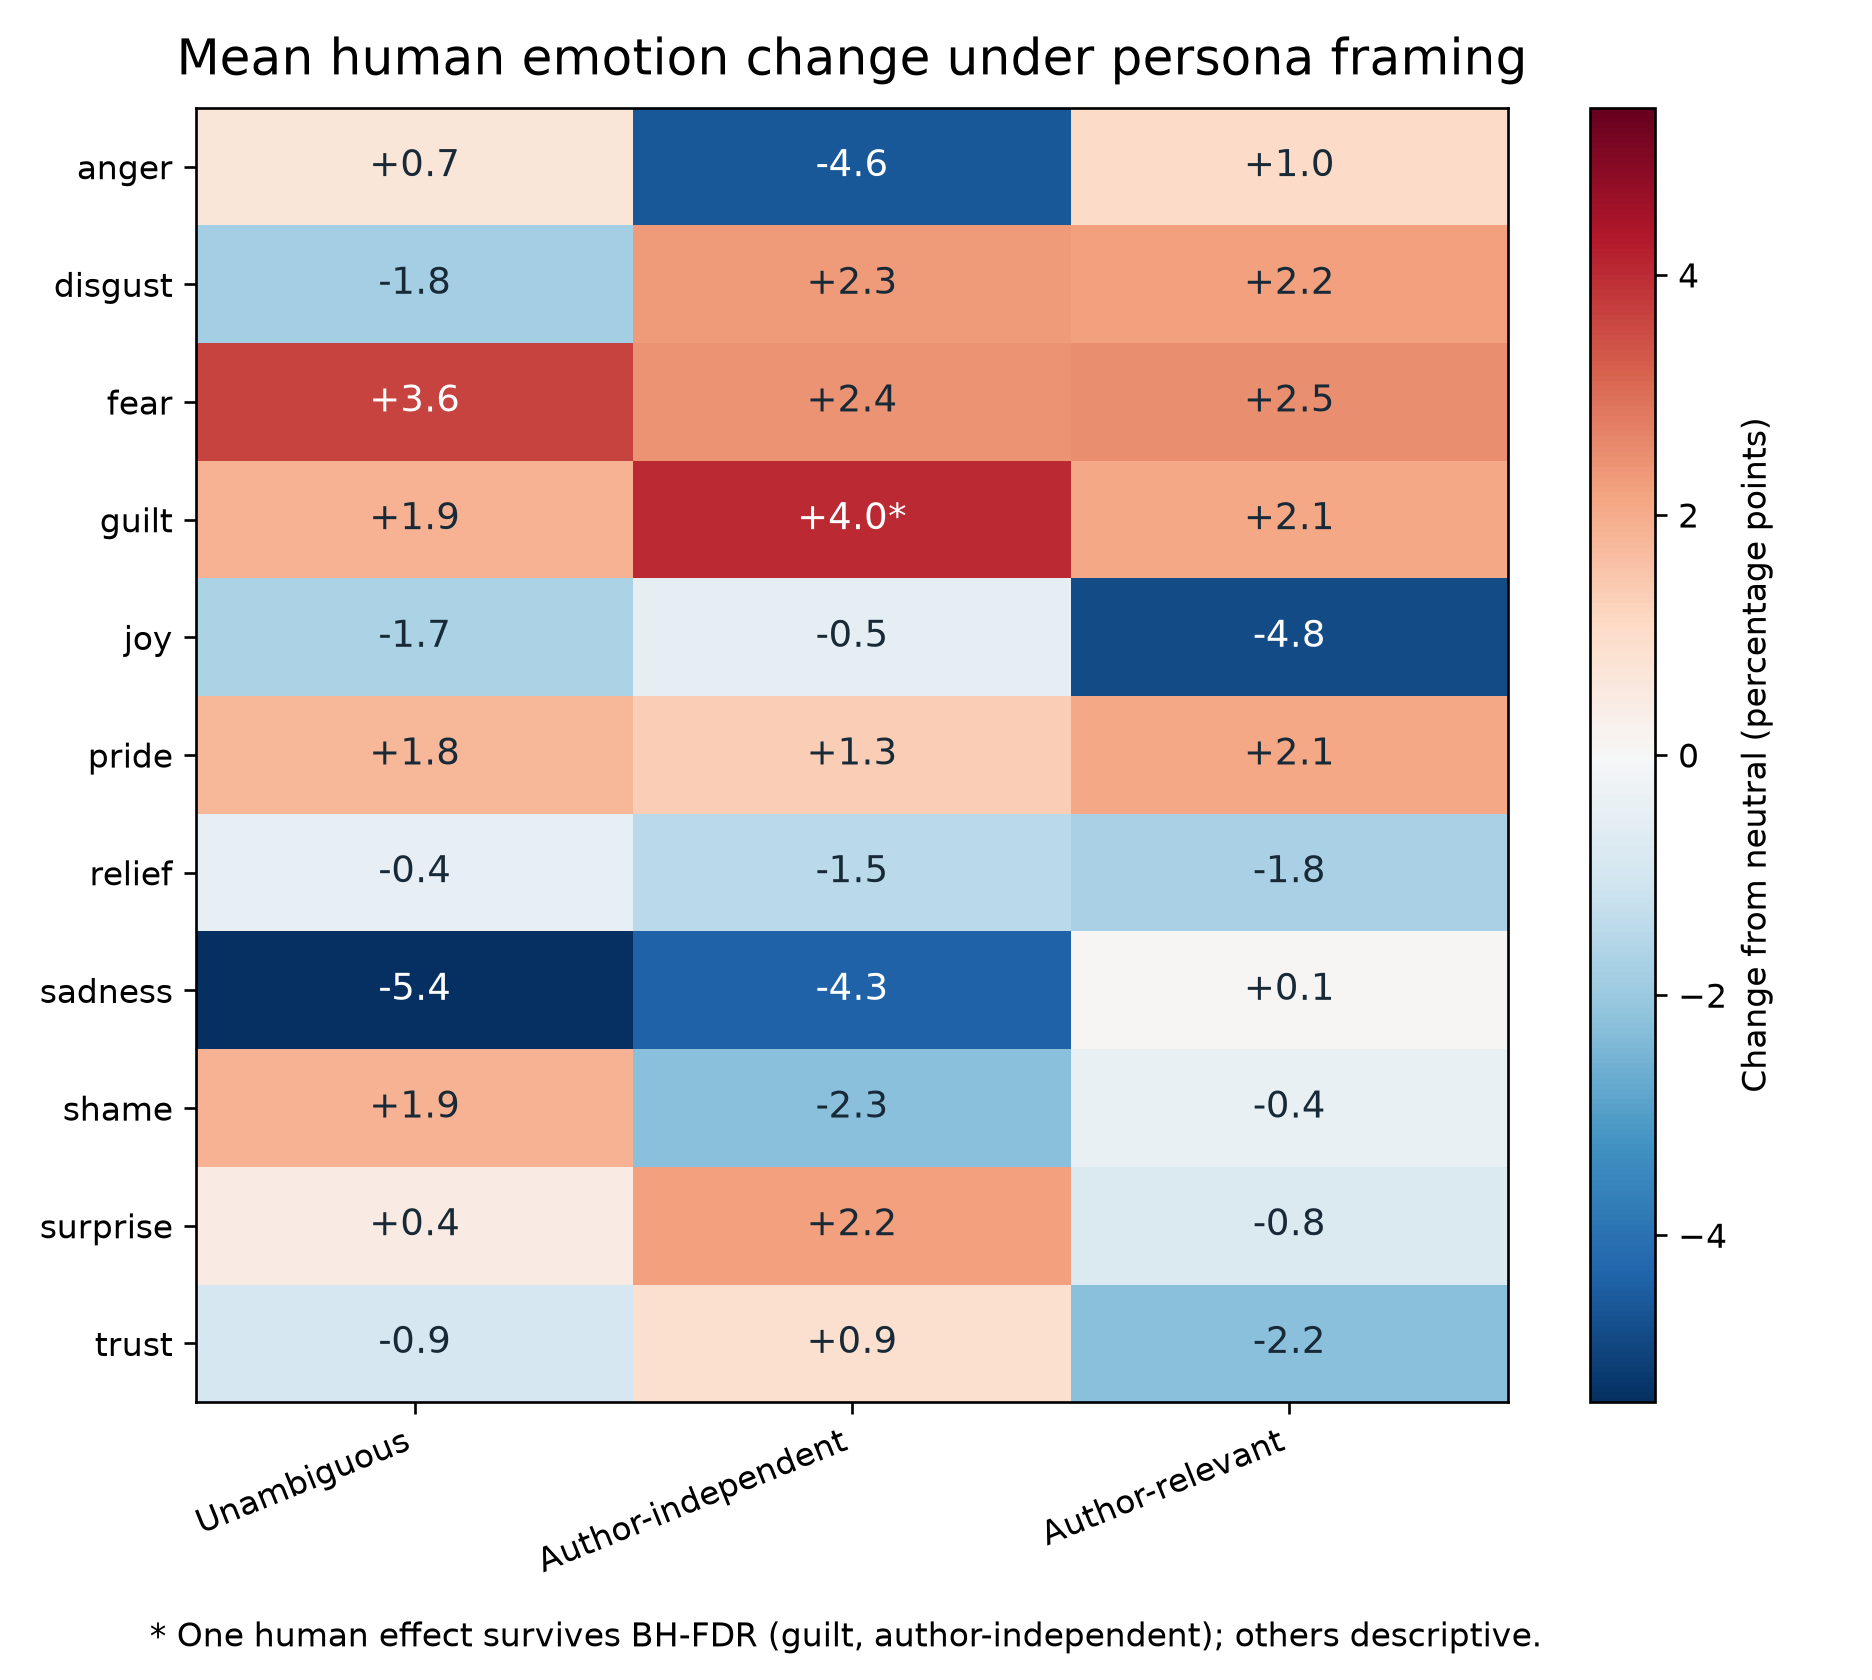
\includegraphics[width=4.6in]{images/fig07_per_emotion_delta_heatmap.png}
    \caption{Mean signed change in probability mass per emotion and category (human, text-level, percentage points).}
    \label{fig:emotionheat}
\end{figure}

\noindent
The biggest descriptive shifts are \textbf{+4.0pp} for \emph{guilt} in the author-independent
category and \textbf{$-$5.4pp} for \emph{sadness} in the unambiguous category, with gains and
losses elsewhere for \emph{fear} and \emph{anger}.

\textbf{The result is different if the test is extended to the model ensemble.} The original analysis covered
only the 33 (category $\times$ emotion) human contrasts. All 66
(source $\times$ category $\times$ emotion) tests were repeated using the identical sign-flip
permutation test and corrected in a single pass using the Benjamini--Hochberg FDR method
(Table~\ref{tab:emotionsig}), yielding \textbf{7 of 66} significant at $q<0.05$. One of the
seven is human: the +4.0pp gain in \emph{guilt} on author-independent texts is significant at this
combined scale ($p_{\text{BH}} = 0.041$), but not on the human-only family tested alone. The other
six are model effects.

\begin{table}[h]
\centering
\footnotesize
\caption{Per-emotion shifts significant under BH-FDR at $q<0.05$ (of 66 tests).}
\label{tab:emotionsig}
\begin{tabular}{llcc}
\hline
\textbf{Source} & \textbf{Category} & \textbf{Emotion (mean change)} & $p_{\text{BH}}$ \\
\hline
Human & Author-Independent & guilt $+4.0$pp & 0.041 \\
LLM   & Unambiguous         & disgust $-0.7$pp & 0.027 \\
LLM   & Unambiguous         & pride $+1.7$pp & 0.009 \\
LLM   & Author-Independent  & joy $-1.9$pp & 0.012 \\
LLM   & Author-Independent  & pride $+1.9$pp & 0.009 \\
LLM   & Author-Relevant     & joy $-5.1$pp & 0.009 \\
LLM   & Author-Relevant     & relief $+3.6$pp & 0.012 \\
\hline
\end{tabular}
\end{table}

\noindent
\textbf{Interpretation.} Of the 33 human cells, the only one to survive correction is the
movement of guilt, already noted above as one of the largest descriptive
shifts (guilt, author-independent), rather than the general ``self-conscious emotions gain,
sadness and anger lose'' pattern visible in the heatmap; the other 32 human cells, including the
numerically larger sadness and fear movements on unambiguous texts, do not survive correction. The
six model effects are not random noise but form a coherent pattern: on both author-independent
and author-relevant texts, the ensemble shifts away from \emph{joy} and towards a more specific
positive emotion (away from \emph{joy} towards \emph{pride}, and away from \emph{joy} towards
\emph{relief}), while on unambiguous texts the ensemble shifts towards \emph{pride} and away from
\emph{disgust}. Given a persona, then, the model ensemble tends to swap a generic positive
emotion for a more specific one rather than bring in threat-related emotions. The result is no
longer reported as a uniform negative finding. It is a small, mostly model-side, directionally
coherent effect, sitting on top of a human per-emotion pattern that this sample size leaves
largely unconfirmed.

\begin{figure}[h]
    \centering
    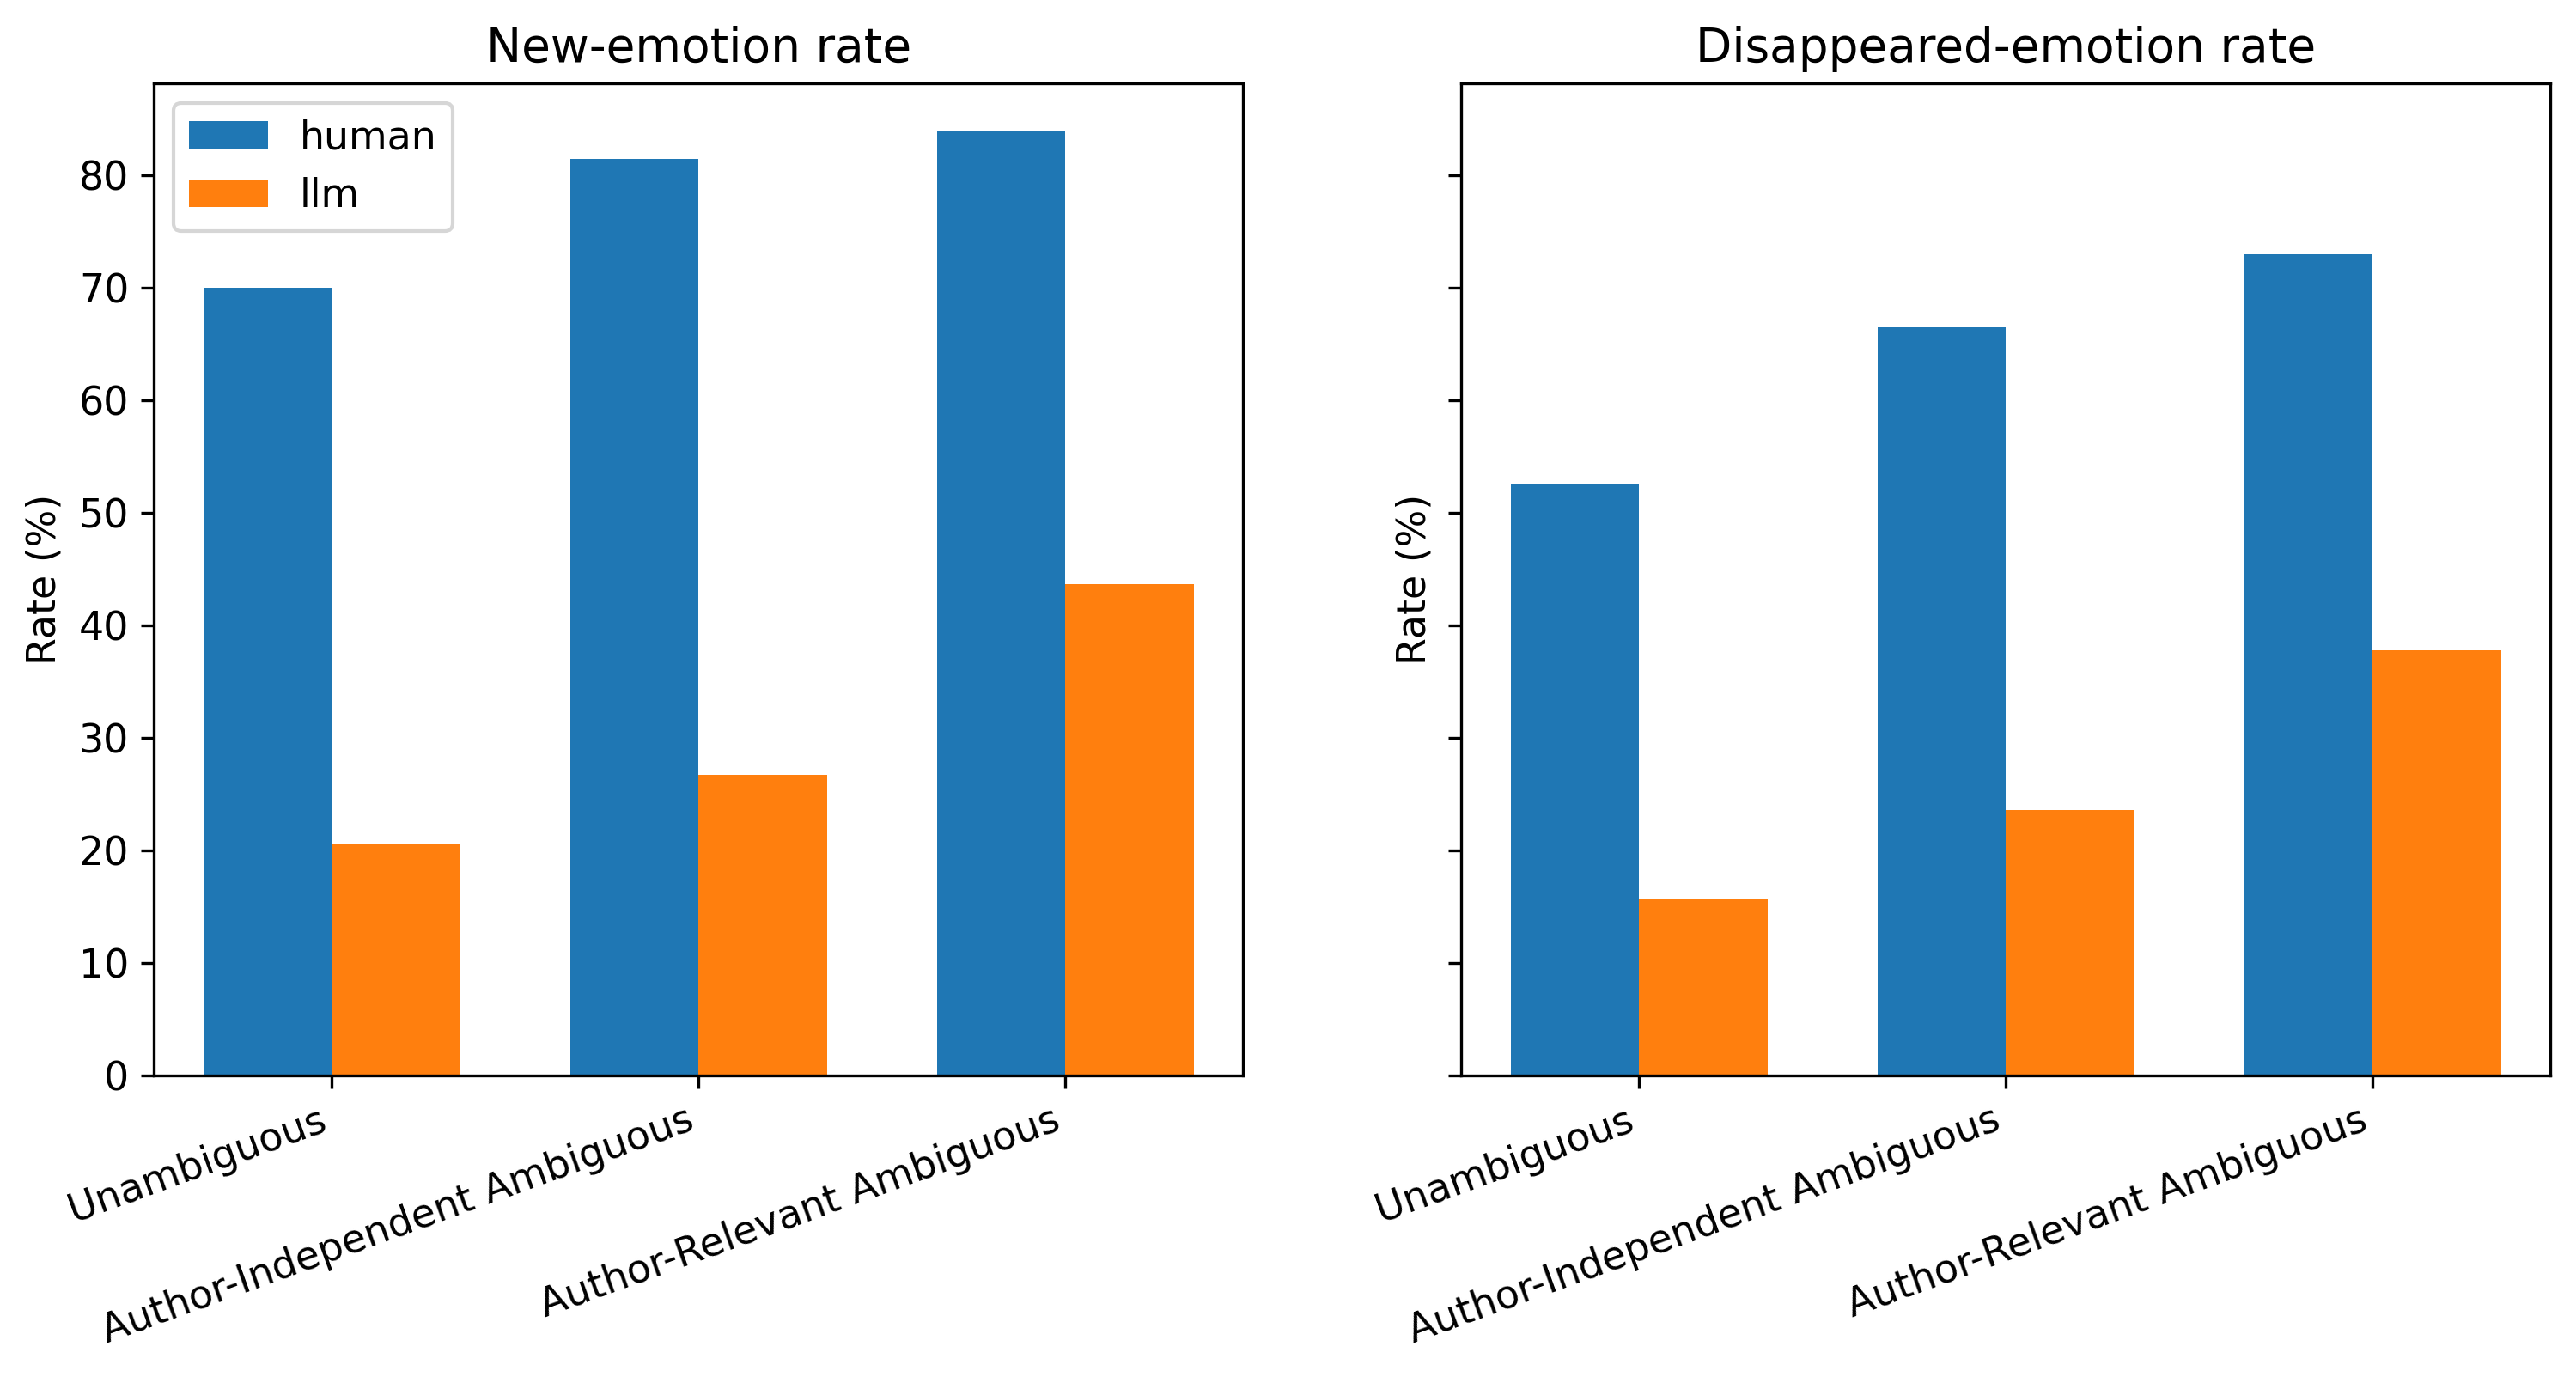
\includegraphics[width=5.0in]{images/fig09_new_disappeared_emotion_rates.png}
    \caption{Rates at which emotions appear or disappear between conditions, by source and category.}
    \label{fig:newdisappeared}
\end{figure}

\noindent
The frequency at which an emotion appears post-framing that was absent beforehand rises with
category for both sources, but is far higher for humans (70.0\%, 81.5\%, 84.0\%) than for the
model ensemble (20.3\%, 26.3\%, 43.4\%). Disappearance rates follow the same ordering (humans
52.5\%, 66.5\%, 73.0\%; models 15.7\%, 23.1\%, 37.3\%). What is being observed here is a change in
the \emph{support}, the set of emotions receiving any vote at all, and not a transition tied to
any specific rater or model; because the human and persona conditions were rated by disjoint
people, no individual vote is ever observed to change. The difference is mostly one of structure,
not behaviour: with only three votes, one human vote landing on a previously unvoted emotion is
enough to change the support, whereas a seven-model ensemble requires the same event across a
larger denominator, so support detection is itself a function of sample size as well as of the
underlying vote distribution.

\section{A Traceable Strong-Shift and Stable-Condition Example}
\label{res:example}

\noindent
Text 2105 is about passing exams; the original emotion word has been removed from the stimulus.
Its neutral human votes are \emph{pride, joy, joy}. The four independent human votes for
Persona~A (a student who had struggled all year and barely managed to pass) are \emph{sadness,
relief, relief, relief}. The two vote sets have disjoint emotion supports, so the TV distance is
$1.0$, a 100\% distributional shift. Persona~B is a high-performing student who expected to pass:
its votes are \emph{pride, joy, joy}, exactly the neutral distribution, giving TV distance $0$.
The case was picked for its observed shift pattern, and the juxtaposition does not
necessarily imply that the persona caused a specific individual to change their answer. Source:
\texttt{data/human\_annotations.csv} (text 2105), with persona wording in
\texttt{data/sampled\_texts.csv}.

For the zero-shot, numbered-list configuration, the OpenAI model outputs \emph{pride} for neutral
framing, \emph{relief} for persona~A, and \emph{pride} for persona~B. The recorded explanations
are, respectively, accomplishment, relief after a difficult year, and success in line with high
expectations (\texttt{data/experiment\_results\_all.csv}, text 2105). These responses indicate
that the explanation field was gathered and that this particular model/configuration is
qualitatively similar to the human contrast, but not that these explanations are a mechanism, and
not that every model/configuration behaves this way.

\section{Does Framing Concentrate or Disperse Interpretation?}
\label{res:entropy}

\noindent
Magnitude and dispersion are different things. A distribution can move a considerable
distance and still end up with one firm new response, or it can spread thin with little movement.
At the text level, the two are empirically close to unrelated in both sources: for humans
$\rho = 0.092$, $p = 0.113$; for the model ensemble $\rho = -0.048$, $p = 0.406$.

A per-text mean entropy change is calculated for each cell and tested with a one-sample Wilcoxon
signed-rank test against a null value of zero (since each text contributes exactly one value, this
avoids the pseudoreplication a per-comparison test would introduce); Benjamini--Hochberg correction
is applied across all six tests.

\begin{figure}[h]
    \centering
    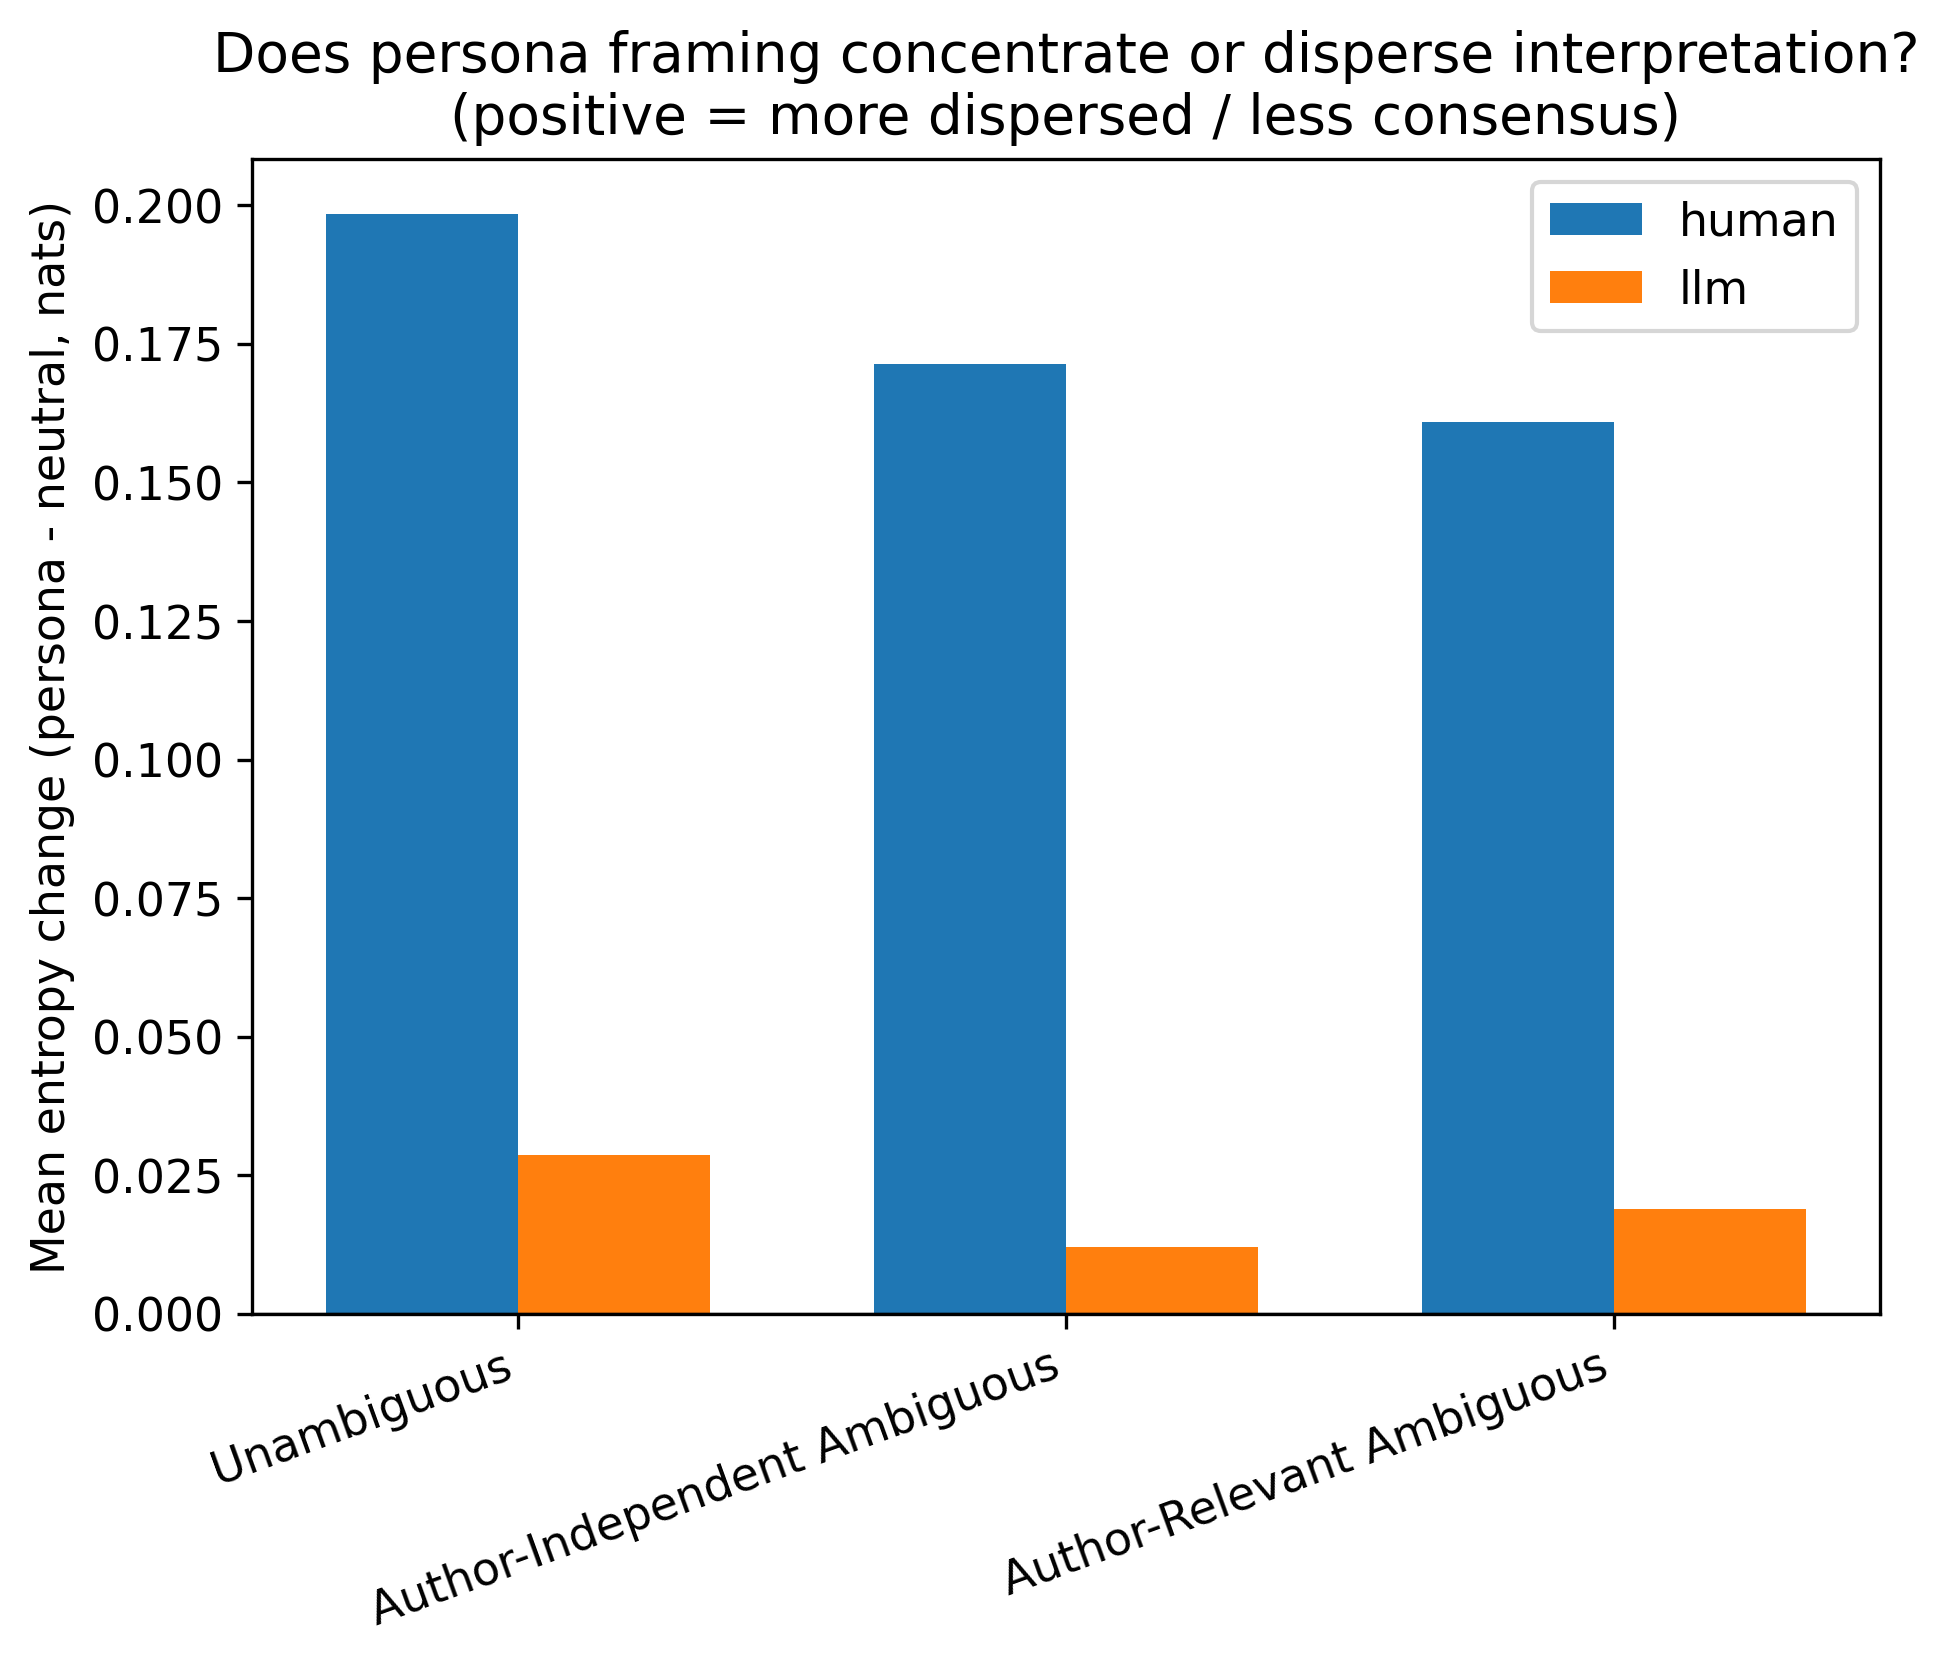
\includegraphics[width=5.0in]{images/fig10_entropy_change_by_category.png}
    \caption{Mean entropy change from neutral to persona framing, by source and category. Positive values indicate greater dispersion.}
    \label{fig:entropy}
\end{figure}

\begin{table}[h]
\centering
\footnotesize
\caption{Entropy change under framing (text-level, BH-FDR corrected across six tests).}
\label{tab:entropy}
\begin{tabular}{llccc}
\hline
\textbf{Source} & \textbf{Category} & \textbf{$\Delta$ entropy} & $p_{\text{BH}}$ & \textbf{Significant} \\
\hline
Human & Unambiguous        & $+0.198$ & 0.0002 & yes \\
Human & Author-Independent & $+0.171$ & 0.0002 & yes \\
Human & Author-Relevant    & $+0.161$ & 0.0030 & yes \\
Model & Unambiguous        & $+0.028$ & 0.226  & no \\
Model & Author-Independent & $+0.012$ & 0.230  & no \\
Model & Author-Relevant    & $+0.021$ & 0.350  & no \\
\hline
\end{tabular}
\end{table}

\noindent
\textbf{Interpretation.} Humans reliably agree \emph{less} among themselves under persona
framing, in all three categories. No dispersion effect is detected on the model ensemble in any
category: it moves its probability mass (Section~\ref{res:h2}) without detectably changing its
internal agreement. These are two separate sets of tests, one significant throughout and one
not. A significant result next to a non-significant one does not by itself show that there is a
statistical difference between the two sources, and that difference was not tested directly. Put
cautiously, human dispersion increases were detected, but model dispersion increases were not.
This hints at an asymmetry that no magnitude-only measure would reveal, but it stops short of a
demonstrated human--model contrast.

A caveat parallels the H4 count-standardisation check (Section~\ref{res:h4counts}): every neutral
human cell rests on exactly three votes, whereas persona cells rest on three to seven, and
plug-in entropy rises mechanically with the number of votes, so part of the raw human entropy
change above is a vote-count artefact rather than framing. Standardising both conditions to three
votes each (\texttt{results/\allowbreak count\_\allowbreak standardisation\_\allowbreak summary.csv}) reduces the mean human entropy
change from $0.177$ to $0.135$ (95\% CI $[0.089, 0.181]$), roughly a quarter smaller, but it
remains clearly positive; the model change is not distinguishable from zero after standardisation
either ($0.013$, CI $[-0.003, 0.029]$).

\section{How Often Does Framing Change Nothing?}
\label{res:zeroshift}

\noindent
In 8.5\% of human comparisons and 40.2\% of model comparisons the persona changed \textbf{nothing
at all} (TV exactly zero). The median TV for humans is 60.0\% and for the ensemble is 14.3\%.

\textbf{Interpretation.} This is not because every cell moves by a moderate amount: the mean
shift of the model ensemble is 18.3\%. A large minority does not move at all, and the rest move
considerably more. This also explains why so many of the cosines in Section~\ref{res:h4direction} are
undefined: a zero delta has no direction. Part of the human--model asymmetry is again structural,
since a seven-way vote has more available states than a three-way vote.

\section{The ``Unchanged'' Category Conceals Movement}
\label{res:dominant}

\noindent
A conventional dominant-label comparison records a change only when the winning emotion flips.
Broken into the five outcomes defined in Section~\ref{impl:dominant}:

\begin{table}[h]
\centering
\footnotesize
\caption{Dominant-set outcomes. These set relationships differ from changes in an alphabetically selected single winner.}
\label{tab:dominant}
\begin{tabular}{lcc}
\hline
\textbf{Outcome} & \textbf{Human} & \textbf{Model ensemble} \\
\hline
Identical set & 34.3\% & 78.9\% \\
Single emotion split into a tie & 17.0\% & 2.6\% \\
Tie resolved to a single emotion & 8.2\% & 3.4\% \\
Partial overlap of two ties & 7.0\% & 0.4\% \\
\hline
\textbf{Fully disjoint top sets} & \textbf{33.5\%} & \textbf{14.8\%} \\
\hline
\end{tabular}
\end{table}

\begin{figure}[h]
    \centering
    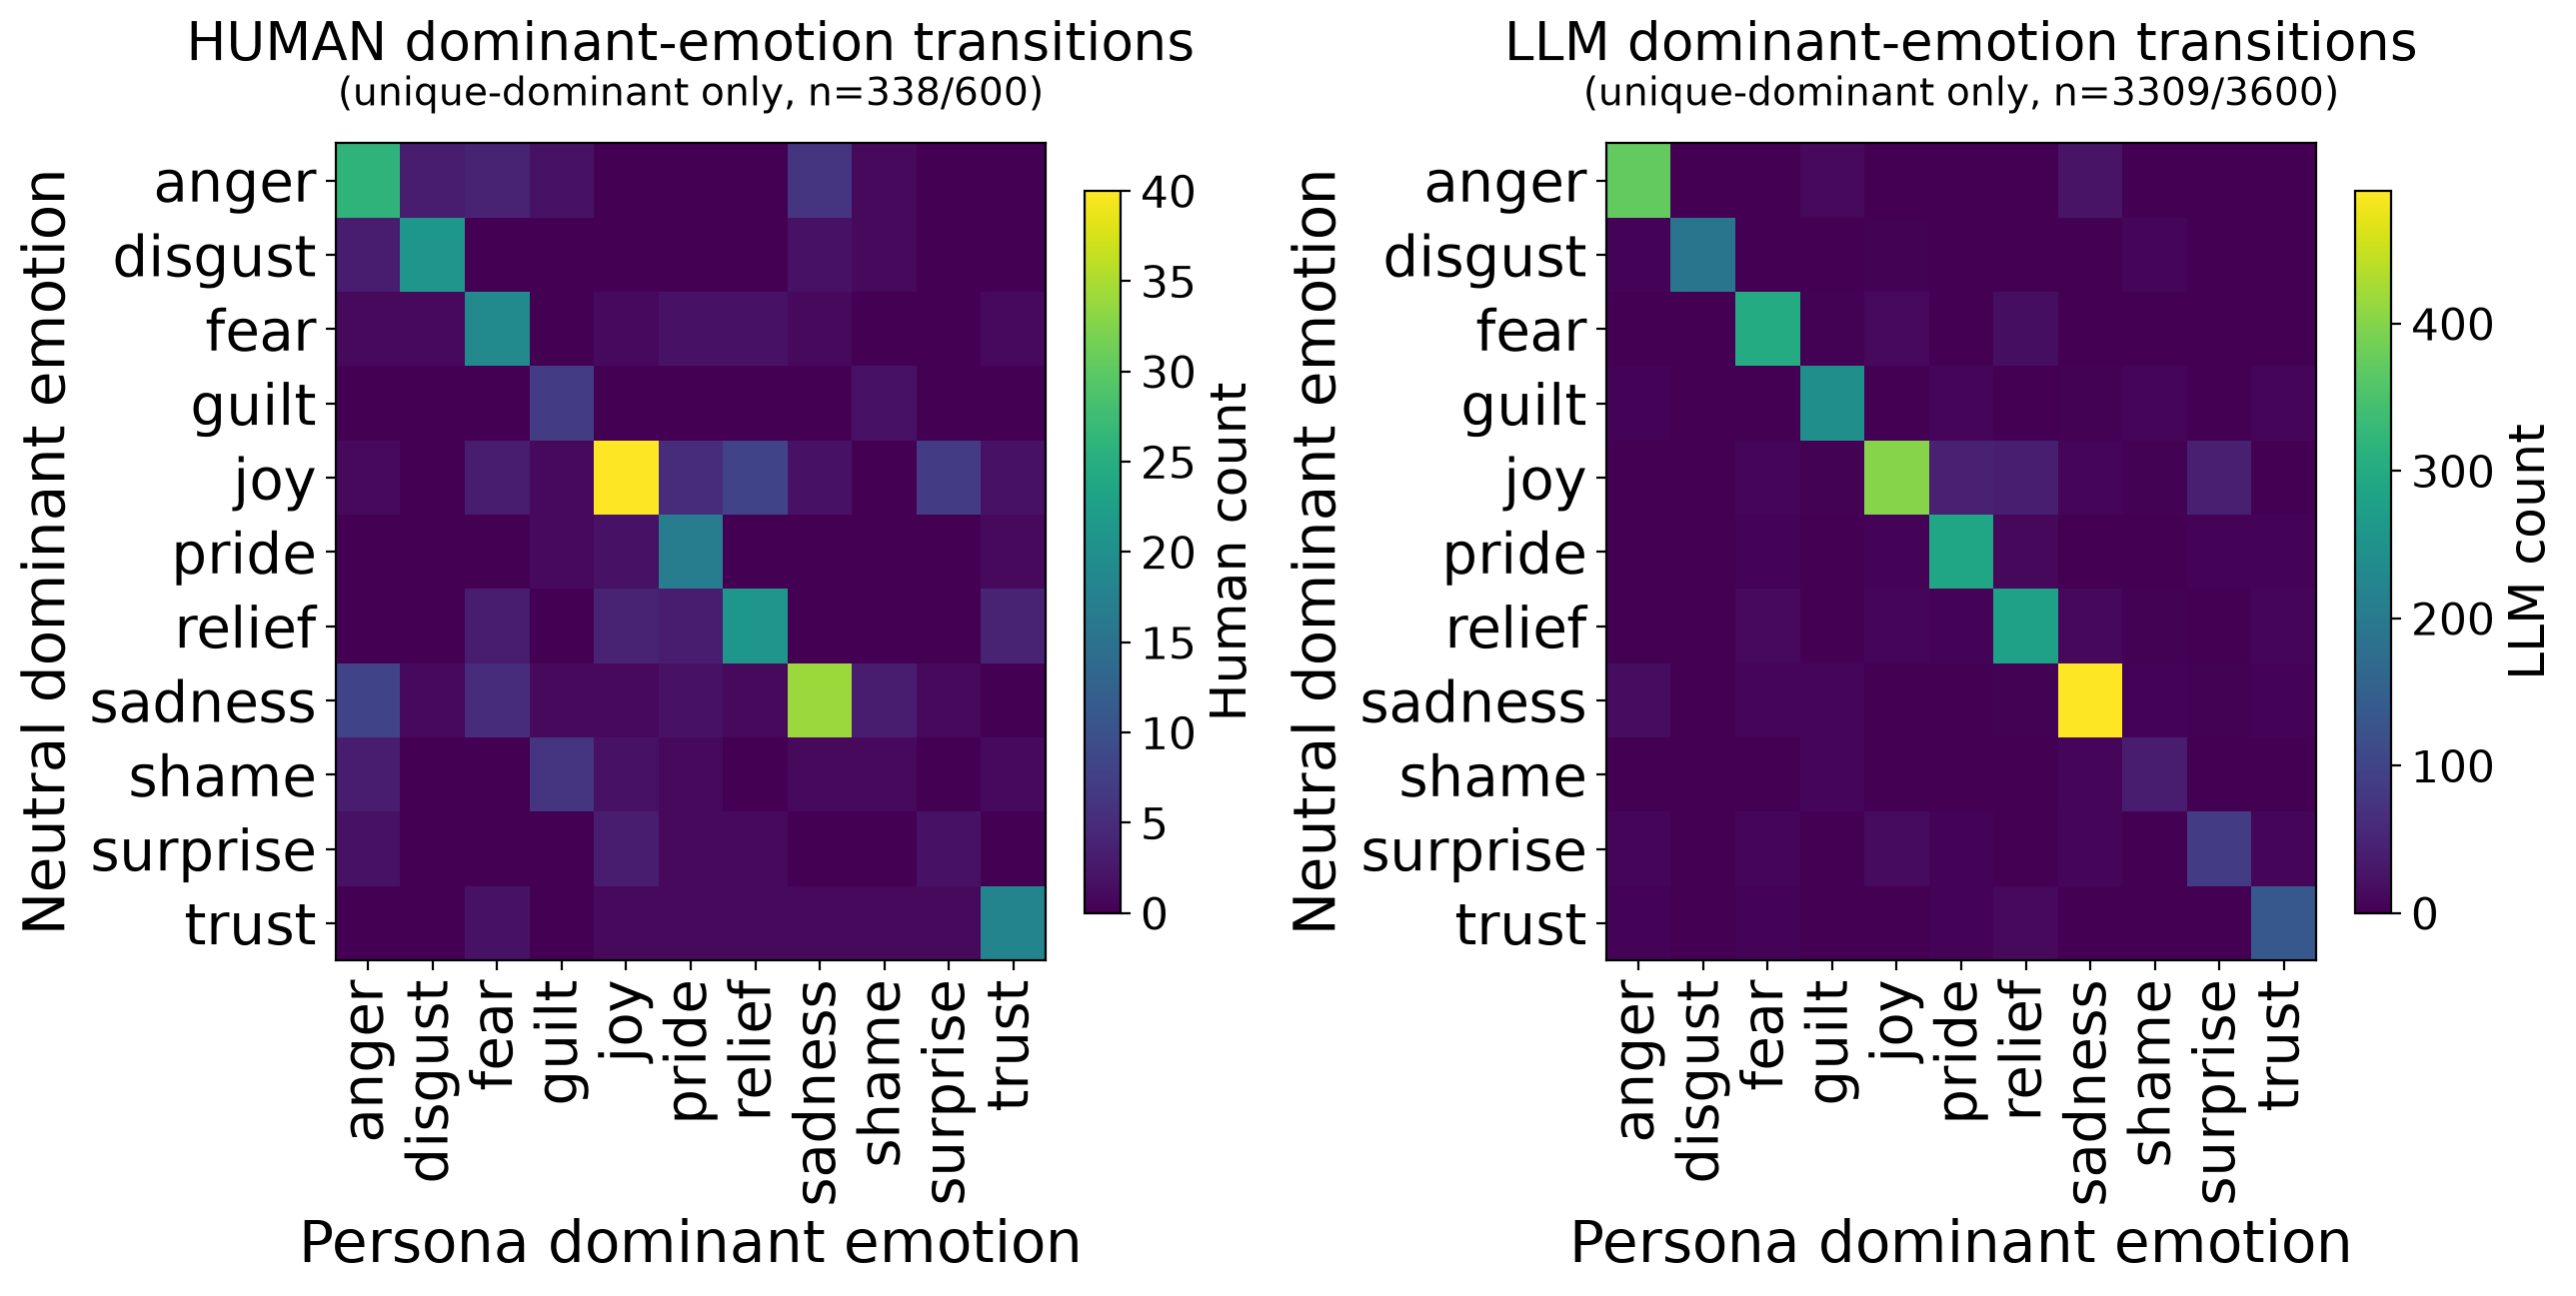
\includegraphics[width=\textwidth]{images/fig08_dominant_transition_matrices.png}
    \caption{Dominant-emotion transition matrices for human and model judgments, restricted to comparisons where both sides have a unique dominant emotion.}
    \label{fig:transitions}
\end{figure}

\noindent
\textbf{Interpretation.} In 33.5\% of the comparisons, human top sets are completely disjoint and
34.3\% are identical, while the remaining 32.2\% involve a tie forming, resolving, or partially
overlapping. The corresponding figures for the model ensemble are 14.8\%, 78.9\%, and 6.3\%. These
are \emph{set} relationships, not the changed/unchanged decisions made by the selected-label
method. That method records 52.8\% of human and 18.4\% of model comparisons as changed
(Section~\ref{res:vectorization}); an overlapping top set can still select a different winner.

\section{Prompt Structure Has No Measurable Effect}
\label{res:prompt}

\noindent
A repeated-measures Friedman test across the six prompt configurations (text-level, $n =
300$) gives $\chi^2 = 7.298$, $p = 0.199$. A test of the selected-label change rate, rather than the
shift, gives $\chi^2 = 1.709$, $p = 0.888$; neither representation detects a prompt-configuration
effect.

\begin{figure}[h]
    \centering
    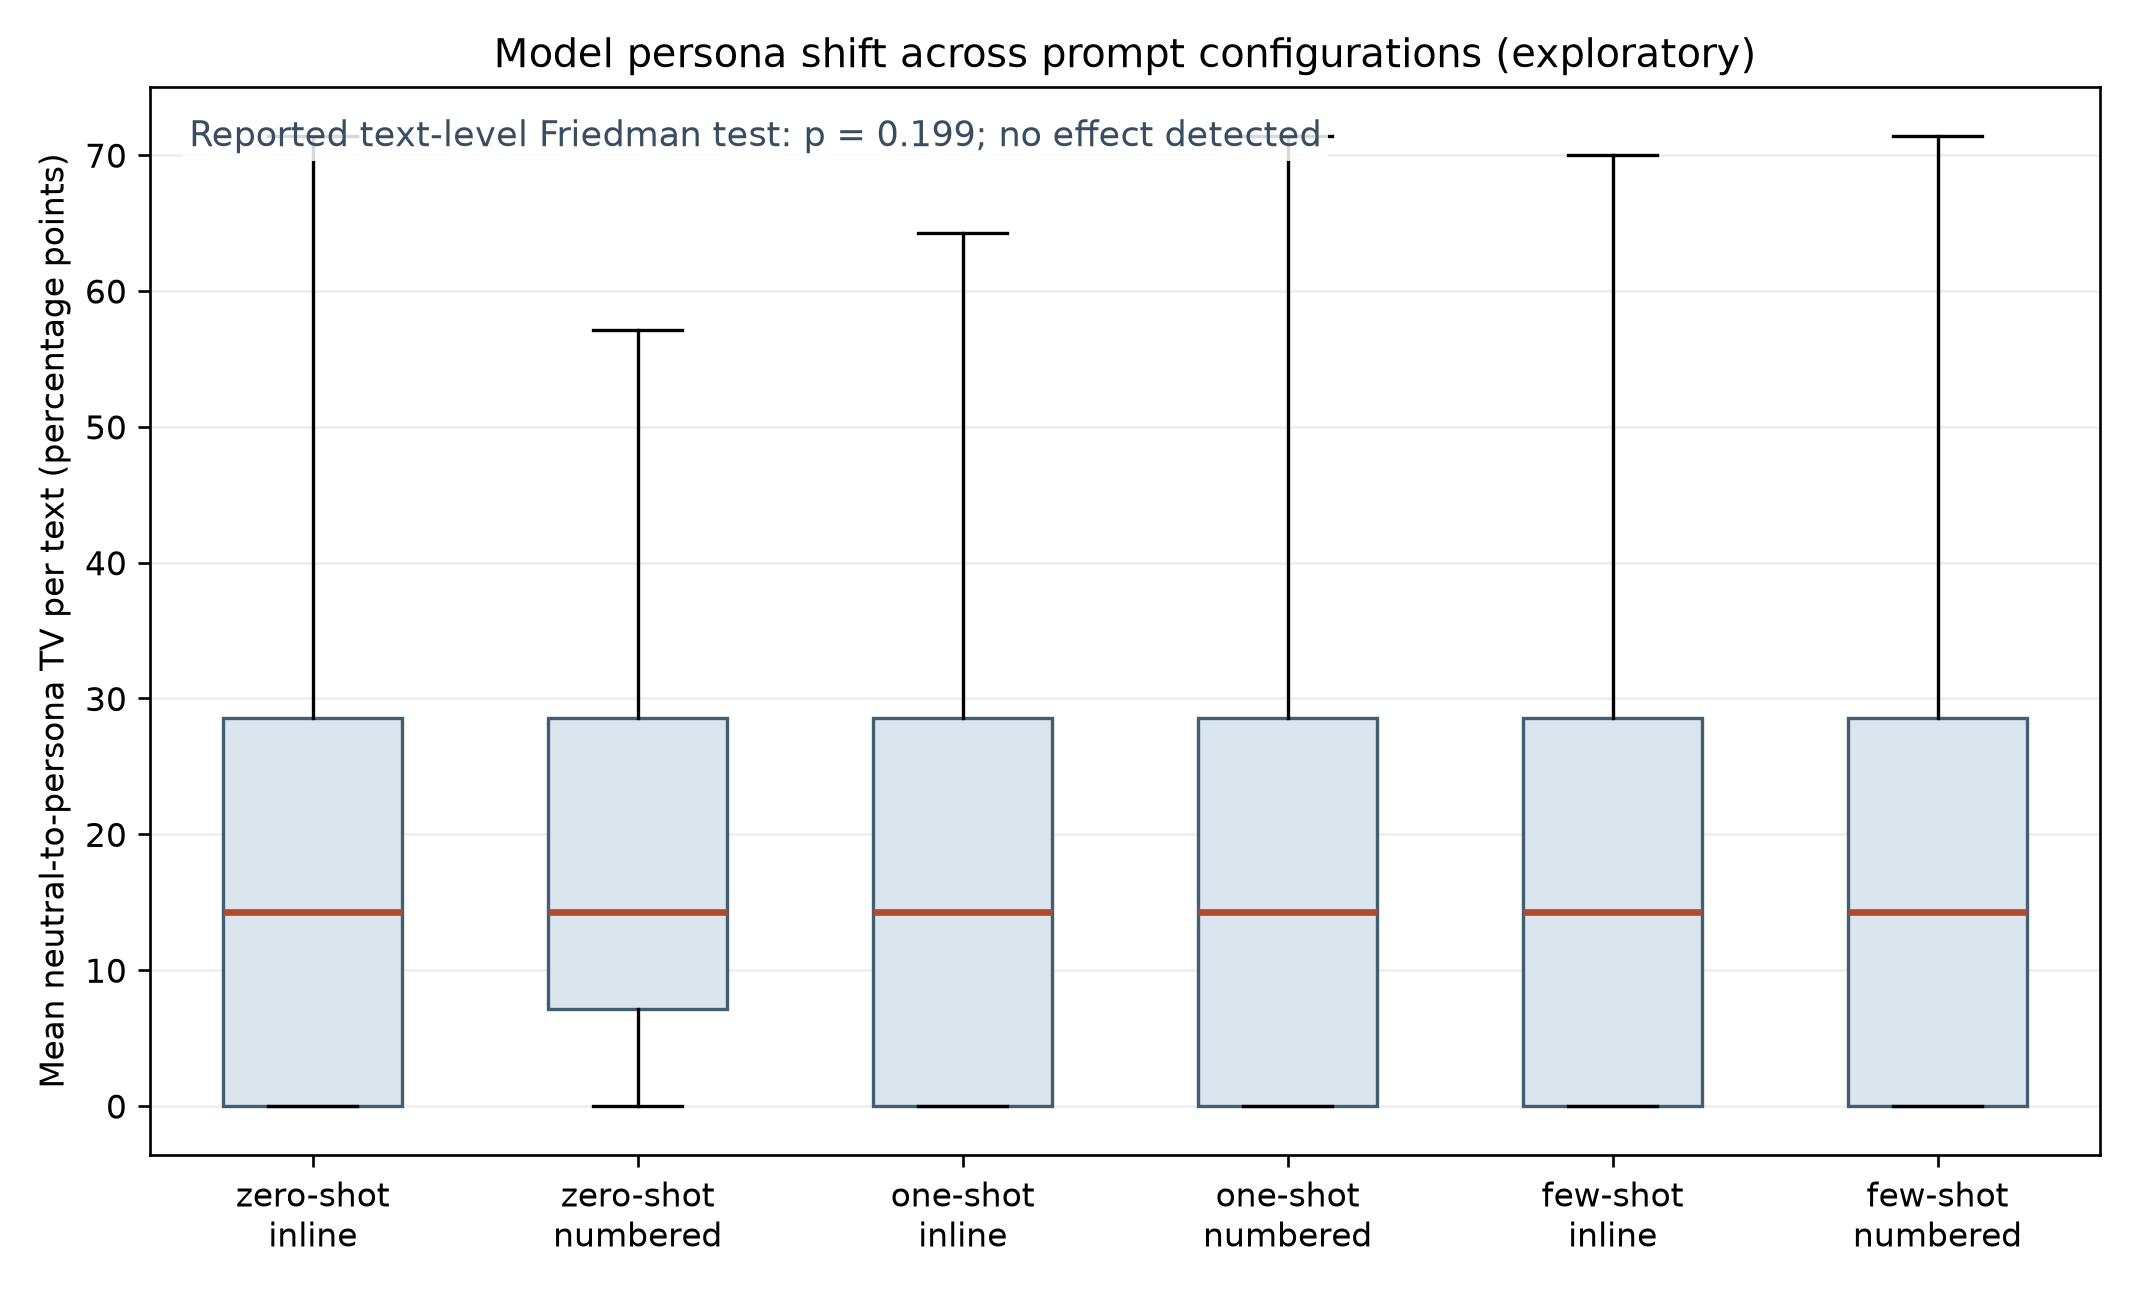
\includegraphics[width=5.0in]{images/fig12_prompt_structure_exploratory.png}
    \caption{Per-text shift magnitude across the six prompt configurations.}
    \label{fig:prompt}
\end{figure}

\noindent
\textbf{Interpretation.} There is no measurable effect on the size of the model framing effect in
this dataset when prompt design (zero-, one- or few-shot) is crossed with either numbered or
inline label presentation. Non-rejection does not establish that prompt configurations are
equivalent. Since the approved proposal contains no numbered hypothesis about prompt structure,
this is a supplementary observation and should not be cited as a test of a formal hypothesis. Its
practical use is as a robustness check: the H2 effect is detectable when the six configurations
are combined, and descriptive effects are present across configurations, but a
configuration-specific equivalence claim is not supported.

\section{Supplementary Check: Human Rating Agreement}
\label{res:agreement}

\noindent
The proposal also requested a check on how well human readers agree with one another. Fleiss'
$\kappa$ asks: \emph{how much more often do readers agree than we would expect based on the
prevalence of each emotion label?} A value of zero is the level of agreement one might expect
from those label frequencies; a larger value indicates greater agreement. It serves only as supporting
description; it is not another hypothesis, nor the main reason for using emotion vectors. It is
calculated for the 754 of 900 text-by-framing cells that have exactly three human
ratings each, separately for each sampled category and framing. All neutral cells have three
ratings, whereas some persona cells have four to seven and are omitted from this particular
statistic. Table~\ref{tab:fleiss} gives both kappa and the number of included texts in parentheses
(source: \texttt{results/\allowbreak human\_\allowbreak interannotator\_\allowbreak agreement\_\allowbreak verified.csv}).

\begin{table}[h]
\centering
\footnotesize
\caption{Human Fleiss' $\kappa$ by sampled category and framing; included cells in parentheses.}
\label{tab:fleiss}
\begin{tabular}{lccc}
\hline
\textbf{Category} & \textbf{Neutral} & \textbf{Persona A} & \textbf{Persona B} \\
\hline
Unambiguous & 0.465 (100) & 0.270 (78) & 0.350 (76) \\
Author-Independent Ambiguous & 0.344 (100) & 0.229 (72) & 0.250 (79) \\
Author-Relevant Ambiguous & 0.294 (100) & 0.177 (75) & 0.159 (74) \\
\hline
\end{tabular}
\end{table}

\noindent
Neutral agreement is highest in the unambiguous pool and lowest in the author-relevant pool. The
persona columns indicate only the exactly-three-vote subset, with different texts included across
the different framings. They therefore do not establish any causal change in agreement, nor do they
replace the within-text framing analysis above.

\section{Summary of Hypothesis Outcomes}
\label{res:summary}

\begin{table}[h]
\centering
\footnotesize
\caption{Summary of hypothesis outcomes.}
\label{tab:summary}
\begin{tabular}{p{2.2cm}p{5.4cm}p{4.6cm}}
\hline
\textbf{Hypothesis} & \textbf{Key evidence} & \textbf{Verdict} \\
\hline
H1 & Author-relevant significant both sides ($p_{\text{Holm}} = 0.0066$, $0.0112$); unambiguous non-significant; author-independent A only, direct A--B inconclusive; selected-label tests: 1 of 6 significant under reverse-alphabetical tie-break, 0 of 6 under alphabetical & Partially supported \\
H2 & Paired test $p_{\text{Holm}} = 0.0002$ both sides; also significant under the selected-label cross-check; 21.3\% of model pairs changed label; generic-author control shows movement for both neutral-to-generic and generic-to-specific steps (not additive components of one total effect) & Supported \\
H3 & Raw: 3 of 3 contrasts Holm-significant. Null-referenced: 0 of 3 & Predicted raw ordering observed; framing-specific contrast inconclusive \\
H4 magnitude & 34.86pp difference, surviving count standardisation ($\approx$34.9 $\rightarrow$ $\approx$33pp); positive text-level covariation (Figure~\ref{fig:h4scatter}) & Supported (magnitudes differ) \\
H4 direction & Mean cosine 0.112, $p = 0.0001$ vs chance pairing & Partially supported \\
Per-emotion (exploratory) & 7 of 66 (source $\times$ category $\times$ emotion) tests significant under BH-FDR: 1 human (guilt), 6 model & Small, mostly model-side effect \\
Prompt structure & Friedman $p = 0.199$ (vector), $p = 0.888$ (selected-label) & No effect detected (exploratory) \\
\hline
\end{tabular}
\end{table}

\begin{figure}[h]
    \centering
    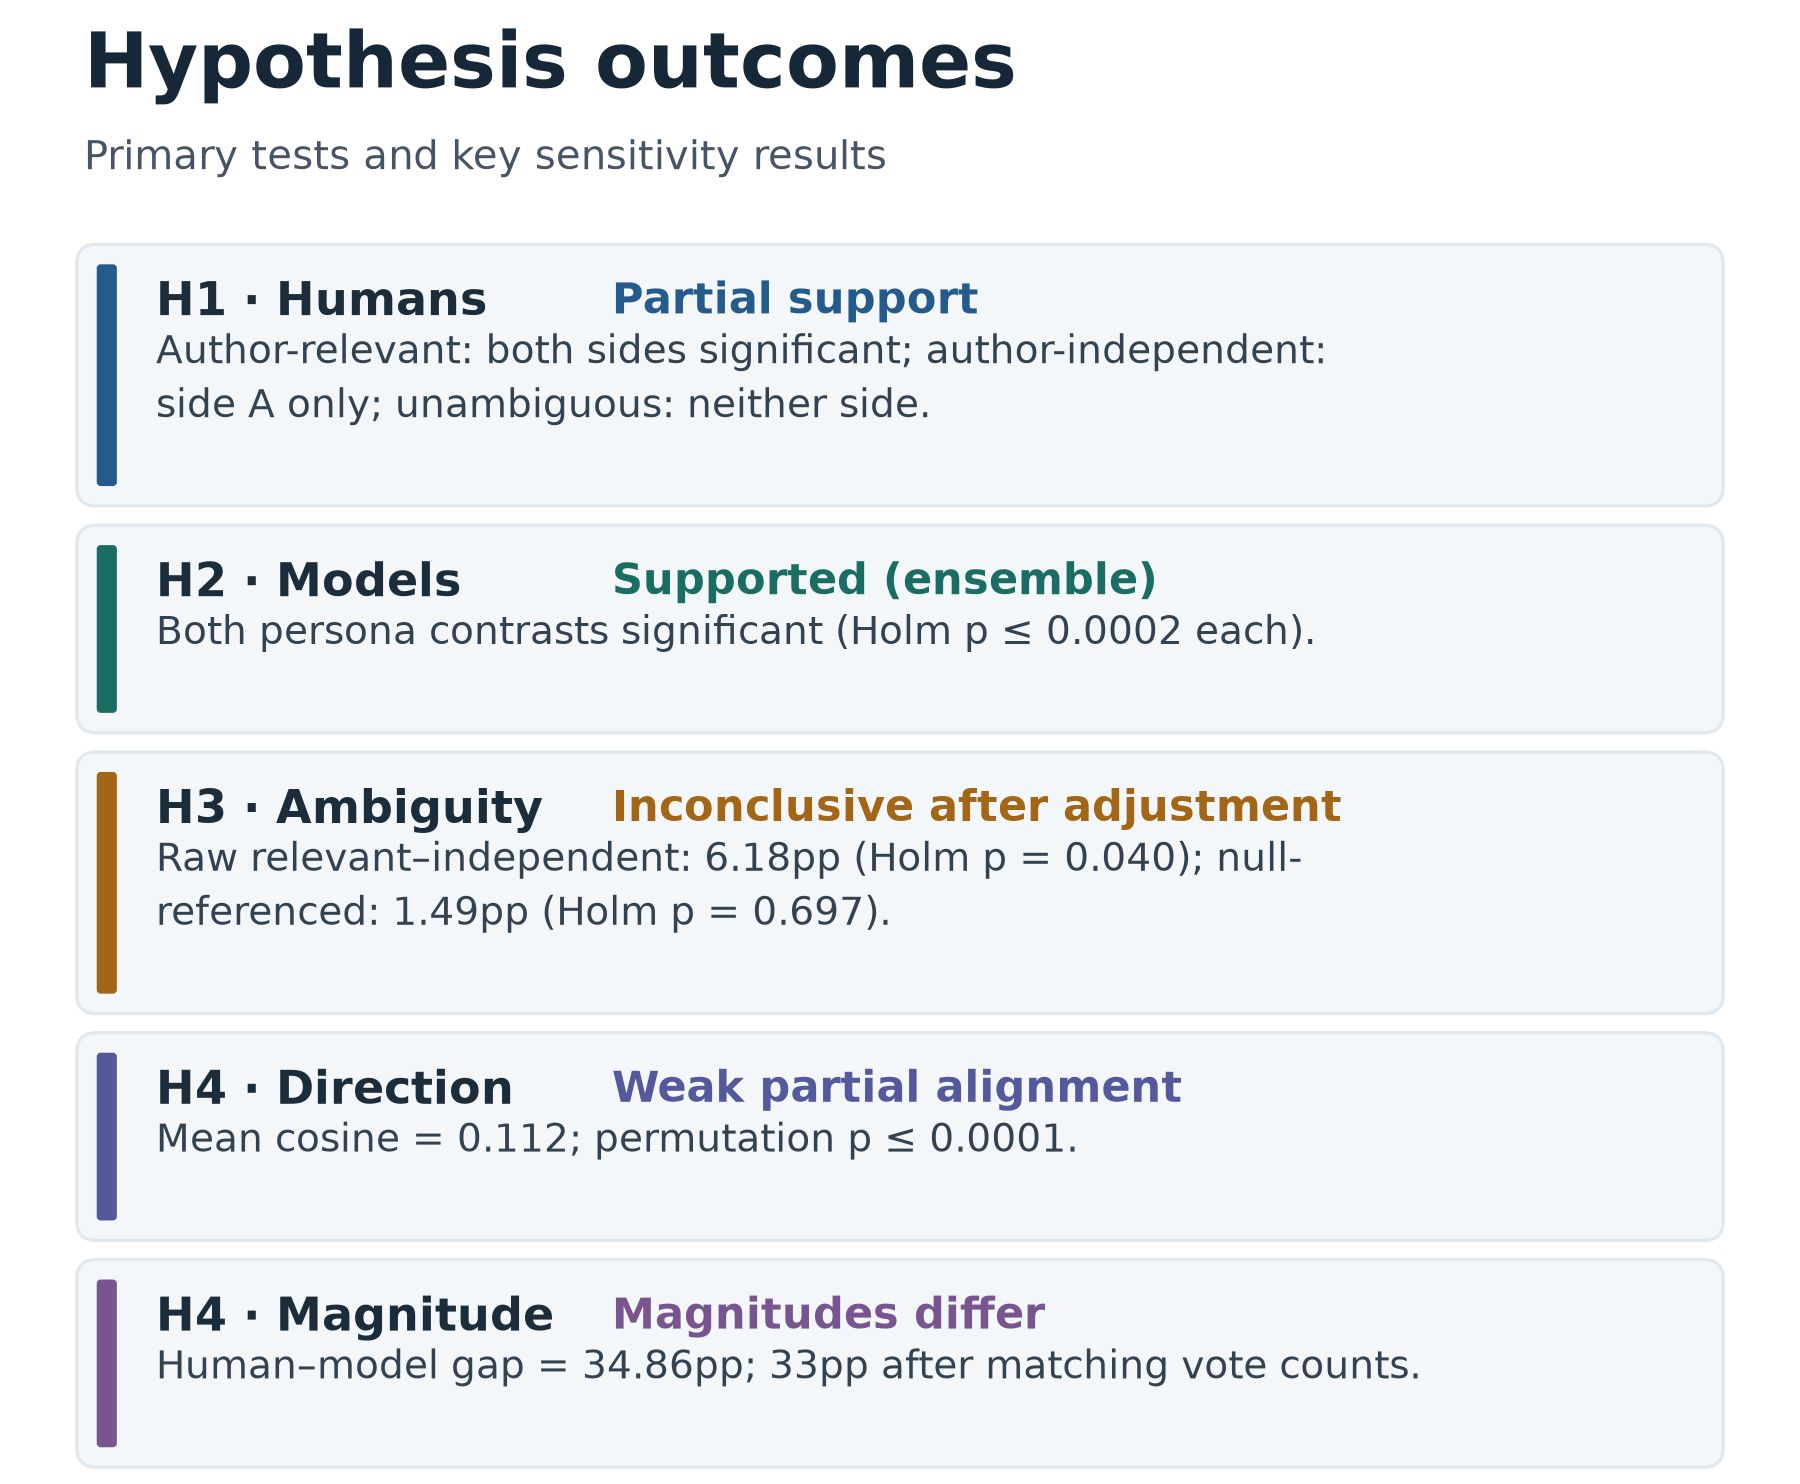
\includegraphics[width=\textwidth]{images/fig13_hypothesis_summary.png}
    \caption{Overview of hypothesis outcomes across the analysis.}
    \label{fig:summary}
\end{figure}
